%%%%%%%%%%%%%%%%%%%%%%%%%%%%%%%
%This is the article LaTeX template for RSC journals
%Copyright The Royal Society of Chemistry 2010
%%%%%%%%%%%%%%%%%%%%%%%%%%%%%%%

\documentclass[8.5pt,twoside,twocolumn]{article}
%\documentclass[12pt]{article}
\oddsidemargin -1.2cm
\evensidemargin -1.2cm
\textwidth 18cm
%\oddsidemargin -0.2cm
%\evensidemargin -1.2cm
%\textwidth 16cm
\headheight 1.0in
\topmargin -3.5cm
\textheight 22cm
\usepackage[super,sort&compress,comma]{natbib} 
\usepackage{mhchem}
\usepackage{siunitx}
\usepackage{times,mathptmx}
% \usepackage{times}
% feel free not to use mathptmx if it causes difficulties
\usepackage{sectsty}
\usepackage{balance} 
\usepackage{comment}
\usepackage{graphicx} %eps figures can be used instead
\usepackage{lastpage}
\usepackage{setspace}
\usepackage[format=plain,justification=raggedright,singlelinecheck=false,font=small,labelfont=bf,labelsep=space]{caption} 
\usepackage{fancyhdr}
\usepackage{multirow}
\usepackage{enumitem}
\usepackage{booktabs}
\usepackage{multicol}
\usepackage{array}
\usepackage{lineno}
\setlength\linenumbersep{0.5cm}
\newcolumntype{H}{>{\setbox0=\hbox\bgroup}c<{\egroup}@{}}
\pagestyle{fancy}


\newcommand{\bra}[2][0]
{\ifthenelse{\equal{#1}{0}}{\left\langle #2 \right|}
{\ifthenelse{\equal{#1}{1}}{\big\langle #2 \big|}
{\ifthenelse{\equal{#1}{2}}{\Big\langle #2 \Big|}
{\ifthenelse{\equal{#1}{3}}{\bigg\langle #2 \bigg|}
{\ifthenelse{\equal{#1}{4}}{\Bigg\langle #2 \Bigg|}
{Error}}}}}
}

% <#2|#3|#4>, #1 gives the size of the bracket
\newcommand{\bracket}[4][0]
{\ifthenelse{\equal{#1}{0}}{\left\langle #2 \middle| #3 \middle| #4 \right\rangle}
{\ifthenelse{\equal{#1}{1}}{\big\langle #2 \big| #3 \big| #4 \big\rangle}
{\ifthenelse{\equal{#1}{2}}{\Big\langle #2 \Big| #3 \Big| #4 \Big\rangle}
{\ifthenelse{\equal{#1}{3}}{\bigg\langle #2 \bigg| #3 \bigg| #4 \bigg\rangle}
{\ifthenelse{\equal{#1}{4}}{\Bigg\langle #2 \Bigg| #3 \Bigg| #4 \Bigg\rangle}
{Error}}}}}
}

% <#2|#3>, #1 gives the size of the bracket
\newcommand{\braket}[3][0]
{\ifthenelse{\equal{#1}{0}}{\left\langle #2 \middle| #3 \right\rangle}
{\ifthenelse{\equal{#1}{1}}{\big\langle #2 \big| #3 \big\rangle}
{\ifthenelse{\equal{#1}{2}}{\Big\langle #2 \Big| #3 \Big\rangle}
{\ifthenelse{\equal{#1}{3}}{\bigg\langle #2 \bigg| #3 \bigg\rangle}
{\ifthenelse{\equal{#1}{4}}{\Bigg\langle #2 \Bigg| #3 \Bigg\rangle}
{Error}}}}}
}

% |#2>, #1 gives the size of the bracket
\newcommand{\ket}[2][0]
{\ifthenelse{\equal{#1}{0}}{\left| #2 \right\rangle}
{\ifthenelse{\equal{#1}{1}}{\big| #2 \big\rangle}
{\ifthenelse{\equal{#1}{2}}{\Big| #2 \Big\rangle}
{\ifthenelse{\equal{#1}{3}}{\bigg| #2 \bigg\rangle}
{\ifthenelse{\equal{#1}{4}}{\Bigg| #2 \Bigg\rangle}
{Error}}}}}
}


\begin{document}
\thispagestyle{plain}
\fancypagestyle{plain}{
\fancyhead[L]{
\includegraphics[height=8pt]{headers/LH}}
\fancyhead[C]{\hspace{-1cm}
\includegraphics[height=20pt]{headers/CH}}
\fancyhead[R]{
\includegraphics[height=10pt]{headers/RH}\vspace{-0.2cm}}
\renewcommand{\headrulewidth}{1pt}}
\renewcommand{\thefootnote}{\fnsymbol{footnote}}
\renewcommand\footnoterule{\vspace*{1pt}% 
\hrule width 3.4in height 0.4pt \vspace*{5pt}} 
\setcounter{secnumdepth}{5}



\makeatletter 
\def\subsubsection{\@startsection{subsubsection}{3}{10pt}{-1.25ex plus -1ex minus -.1ex}{0ex plus 0ex}{\normalsize\bf}} 
\def\paragraph{\@startsection{paragraph}{4}{10pt}{-1.25ex plus -1ex minus -.1ex}{0ex plus 0ex}{\normalsize\textit}} 
\renewcommand\@biblabel[1]{#1}            
\renewcommand\@makefntext[1]% 
{\noindent\makebox[0pt][r]{\@thefnmark\,}#1}
\makeatother 
\renewcommand{\figurename}{\small{Fig.}~}
\sectionfont{\large}
\subsectionfont{\normalsize} 

\fancyfoot{}
\fancyfoot[LO,RE]{\vspace{-7pt}
\includegraphics[height=9pt]{headers/LF}}
\fancyfoot[CO]{\vspace{-7.2pt}\hspace{12.2cm}
\includegraphics{headers/RF}}
\fancyfoot[CE]{\vspace{-7.5pt}\hspace{-13.5cm}
\includegraphics{headers/RF}}
\fancyfoot[RO]{\footnotesize{\sffamily{1--\pageref{LastPage} ~\textbar  \hspace{2pt}\thepage}}}
\fancyfoot[LE]{\footnotesize{\sffamily{\thepage~\textbar\hspace{3.45cm} 1--\pageref{LastPage}}}}
\fancyhead{}
\renewcommand{\headrulewidth}{1pt} 
\renewcommand{\footrulewidth}{1pt}
\setlength{\arrayrulewidth}{1pt}
\setlength{\columnsep}{6.5mm}
\setlength\bibsep{1pt}

%\linenumbers
\noindent\LARGE{\textbf{
%Using Conventional Density Functionals to Simulate X-Ray Absorption Spectra: With Applications to Adenine and Thymine Photoabsorption Spectra
Simulation of X-Ray Absorption Spectra with Orthogonality Constrained Density Functional Theory
}}
\vspace{0.6cm}

\noindent\large{\textbf{Wallace D. Derricotte and Francesco A. Evangelista$^{\ast}$}}\vspace{0.5cm}
%Please note that \ast indicates the corresponding author(s) but no footnote text is required. 


\noindent\textit{\small{\textbf{Received Xth XXXXXXXXXX 20XX, Accepted Xth XXXXXXXXX 20XX\newline
First published on the web Xth XXXXXXXXXX 200X}}}

\noindent \textbf{\small{DOI: 10.1039/b000000x}}
\vspace{0.6cm}
%Please do not change this text.

\noindent \normalsize{Orthogonality Constrained Density Functional Theory (OCDFT) is used to compute excited states relevant to core-level spectroscopy, specifically the high lying excited states crucial to simulate near-edge X-ray absorption spectra (NEXAS). Density functional techniques that employ conventional exchange-correlation (XC) functionals routinely underestimate these excited states. This underestimation necessitates an artificial shift in the resulting spectra in order to make a comparison with experimental data. Here, we prove that OCDFT can accurately compute core excitation energies using conventional density functionals by assessing it's performance over a benchmarking test set of 40 core excitations. We utilize standard XC functionals (B3LYP, BLYP, PBE0), and compare these results with experimental data and time dependent density functional theory computations. We reveal the latent ability of OCDFT by simulating the gas-phase near-edge spectra of adenine and thymine. Our computations are consistent with previous NEXAS studies performed on these molecules and show dominant $\pi^*$ character mixed with definitive Rydberg transitions. The experimentally observed peak intensities are in excellent agreement with our calculated oscillator strengths, showing that OCDFT can accurately compute transition dipole moments.}
\vspace{0.5cm}

%\doublespacing
\section{Introduction}
The advent of synchrotron light sources created a strong resurgence of spectroscopy in the X-ray region. \cite{mcmillan_synchrotronproposed_1945} Near-edge X-ray absorption spectroscopy (NEXAS) is a useful experimental technique to probe the local electronic and geometrical structure in a variety of molecular environments.
The most dominant feature of NEXAS spectra, the \textit{near edge}  (see Fig.~\ref{fig:nexas-illustration}), is composed of the excitations of core-electrons to unoccupied orbitals.
In particular, excitations from 1s orbitals are atom-specific and sensitive to the local chemical environment.
Thus, NEXAS spectra can provide information about the chemical composition and the electronic structure of molecules.
NEXAS has been successfully applied to large biological systems, \cite{hua_refinement_2010} small molecules in the gas phase,\cite{contini_gas-phase_2001} organic thin-films,\cite{hahner_near_2006} and semiconducting materials.\cite{guo_electronic_2011} This wide range of applications is possible because synchrotron light sources can span an energy range that goes from a few electron volts (eVs) \cite{feneberg_synchrotron-based_2011} to hundreds of MeVs.\cite{nakazato_observation_1989}

\begin{figure}
\centering
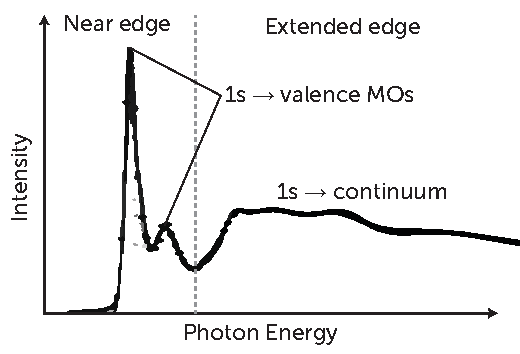
\includegraphics[width=8.8cm]{NEXASIllustration.pdf}
\caption{Example of a X-ray photoabsorption spectrum (XAS).  The near edge, located in the low energy region, consists of excitations of core electrons to valence orbitals.  These transitions are sensitive to the chemical environment surrounding the excited atom.  The high energy region of the spectrum results from excitations of core electrons to the continuum.}
\label{fig:nexas-illustration}
\end{figure}

As NEXAS experiments are becoming more feasible, there is a growing need to develop accurate theoretical approaches to aid the interpretation of experimental spectra.
%In order for a method to properly replicate and analyze NEXAS spectra, it must demonstrate accuracy in describing core-electron excitations. 
Calculations of NEXAS spectra are challenging, and require computational methods that explicitly account for the excitations of core-level electrons, orbital relaxation effects, and electron correlation. \cite{coriani_coupled-cluster_2012} Several theoretical approaches have been adapted to compute core-valence excitations, including: scaled-opposite-spin configuration interaction singles with perturbative doubles [SOS-CIS(D)],\cite{asmuruf_calculation_2008} second-order algebraic digrammatic construction [ADC(2)],\cite{schirmer_beyond_1982,trofimov_efficient_1995} multiple scattering X$_\alpha$ methods, \cite{sheehy_correlation_1989} a maximum overlap $\Delta$SCF approach, \cite{besley_self-consistent-field_2009} transition potential theory,\cite{triguero_calculations_1998} coupled-cluster response theory, \cite{coriani_coupled-cluster_2012} and time-dependent density functional theory (TDDFT).\cite{stener_time_2003} Among these methods, TDDFT is perhaps the most attractive option because of its reduced computational cost and ability to calculate multiple excited states.

TDDFT is a rigorous extension of the DFT ground-state formalism,\cite{runge_density-functional_1984} and it is regarded as the method of choice to treat electronic excited states within a density functional framework.
%Within the framework of density functional theory, TDDFT is regarded as the method of choice to treat electronic excited states because it is a rigorous extension of the ground-state formalism.\cite{runge_density-functional_1984}
 When applied in conjunction with frequency-independent exchange-correlation potentials, TDDFT yields accurate excitation energies for low-lying excited states. For example, the TDDFT benchmark study of Silva-Junior and co-workers\cite{silva-junior_benchmarks_2008} on 28 organic molecules, showed that singlet and triplet excitation energies can be calculated with a mean average error (MAE) of 0.27 eV and 0.44 eV, respectively. However, Besley et al.\cite{besley_self-consistent-field_2009} showed that TDDFT core excitations computed with conventional exchange-correlation functionals grossly underestimate experimental results, yielding a MAE of 20.2 eV. It is customary to remedy this deficiency of TDDFT by shifting the position of computed spectra by an amount that minimizes the difference between the computational and experimental peak features. For example, a study done by DeBeer, Petrenko, and Neese\cite{debeer_george_prediction_2008} showed that it is necessary shift the TDDFT Fe near-edge spectra of different iron complexes by 171.3 eV in order to correct the spectra.
 TDDFT core-valence excitation energies can also be improved by introducing self-interaction corrections (SIC),\cite{tu_core_2007} or range separated hybrid functionals in which the amount of long and short range Hartree--Fock exchange is reparametrized.\cite{besley_time-dependent_2009, nakata_time-dependent_2006} This is often the limiting factor for studying the edge structure of many chemical systems since the optimal amount of Hartree--Fock exchange is system dependent.\cite{capano_role_2013,besley_time-dependent_2007,besley_time-dependent_2010}

Given the difficulties encountered by TDDFT in computing charge-transfer excited states\cite{dreuw_failure_2004} and the self interaction error that afflicts traditional density functionals, this failure is to be expected.
Work by Peach et al. \cite{peach_excitation_2008} suggests that there is a direct correlation between the accuracy of TDDFT and the degree of spatial overlap ($\Lambda$) between the occupied and virtual orbitals involved in the excitation. Low orbital overlap is a characteristic feature of both charge transfer excitations and core excitations, with the relationship between accuracy and orbital overlap being persistent through core excitations as well. \cite{besley_time-dependent_2009}
The inaccuracy of TDDFT for excitations with low values of $\Lambda$ has been attributed to the incorrect asymptotic behavior of the exchange-correlation potential and self-interaction error.\cite{peach_excitation_2008}

A general method that can systematically produce accurate core-excitation energies with traditional hybrid density functionals is highly desirable. The maximum overlap method (MOM) \cite{besley_self-consistent-field_2009} combined with a $\Delta$SCF treatment of core-valence excitations is able to obtain highly accurate excitation energies using conventional functionals. However, this procedure is not guaranteed to avoid the problem of variational collapse---albeit MOM ameliorates the difficulties encountered by a straightforward $\Delta$SCF procedure---and has not been generalized to multiple excited states of the same symmetry.

The goal of this work is to find cost-effective alternative theories to TDDFT that can be used to simulate NEXAS spectra.
Orthogonality constrained density functional theory (OCDFT)\cite{evangelista_orthogonality_2013}  was rigorously derived from a variational time-independent formulation of excited state DFT.
It builds upon previous successful efforts to formulate variational excited state DFT, such as: the $\Delta$SCF procedure, \cite{kowalczyk_assessment_2011,ziegler_calculation_1977} constrained DFT,\cite{wu_constrained_2006} stationary state DFT, \cite{gorling_density-functional_1999}  constricted variational density functional theory (CV-DFT), \cite{ziegler_relation_2009,ziegler_application_2011,krykunov_self-consistent_2013,ziegler_implementation_2012}
perturbative constrained excited state DFT,\cite{baruah_dft_2009,olguin_effect_2013,zope_charge_2012} ensemble DFT,\cite{theophilou_energy_1979,fritsche_generalized_1986,gross_rayleigh-ritz_1988,gross_density-functional_1988} and variational time independent DFT (TI-DFT). \cite{levy_variational_1999,nagy_variational_2001}
Formally OCDFT may be viewed as bridging constrained and constricted variational DFT.  Its main advantages are: 1) it has favorable accuracy/cost ratio, similar to that of ground state DFT, 2) it is numerically robust and avoids variational collapse, and 3) it yields excitation energies that are spin adapted.
Benchmark computations\cite{evangelista_orthogonality_2013} show that valence excitation energies computed with OCDFT have error metrics comparable to that of TDDFT.  In addition, OCDFT has the ability to accurately compute charge transfer excitation energies regardless of the amount of Hartree-Fock exchange present in the exchange-correlation functional.

This work introduces two new developments of OCDFT that are necessary for the simulation of near-edge X-ray  absorption spectra.
First, we formulate an OCDFT algorithm that can be used to compute core-valence excitation energies.  This new method is assessed over a test set that includes 13 molecules with 40 unique core-electron excitations.
Second, we discuss one approach to extend OCDFT to multiple excited states of the same symmetry.
We demonstrate the potential of this new method with computations of the gas-phase near-edge spectra of adenine and thymine.


\section{Theory}
In this section we provide a brief summary of orthogonality constrained density functional theory along with the necessary extension to multiple excited states (for the full details of the OCDFT derivation we refer the reader to Ref.\citenum{evangelista_orthogonality_2013}).
OCDFT builds upon the time-independent variational DFT approach developed by Ayers, Levy, and Nagy.\cite{ayers_time-independent_2012}
To each electronic state [$\Psi^{(n)}, n=0,1,\ldots$] of a $N$-electron system, we associate a density functional $E^{(n)}[\rho]$:
\begin{equation}
E^{(n)}[\rho] = \min_{
\substack{
\Psi \rightarrow \rho\\
\Psi\bot\Psi^{(k)}
}
}
\bra{\Psi}\hat{H}\ket{\Psi},
\;\;\; k = 1,\ldots,n-1.
\end{equation}
$E^{(n)}[\rho]$ searches for the wave function that minimizes the energy subject to density constraint and at the same time enforces the orthogonality between $\Psi$ and the first $n-1$ \textit{exact} electronic states:

OCDFT starts from the time-independent approach based on the functionals $E^{(n)}[\rho]$ to produce a computationally viable method.
%with wave function $\Phi^{(n)}$ and density $\rho_s^{(n)}$ 
%Starting from this theory, it is possible to introduce a generalization of the Kohn--Sham scheme that enables us to express variational excited state density functionals in terms of $\phi^{(n)}$, the occupied orbitals of electronic states $n$.
The first step consists in defining a generalized Kohn--Shame scheme that, for each electronic state $\Psi^{(n)}$,  defines an auxiliary system of noninteracting electrons with wave function $\Phi^{(n)}$ and density $\rho_s^{(n)}$.  The density of state $\Phi^{(n)}$ is assumed to be equal to the exact density of state $\Psi^{(n)}$, which we indicate with $\rho^{(n)}$.
In addition, we assume that the auxiliary wave functions are orthogonal, that is:
\begin{equation}\label{eq:orthogonality_condition}
\braket[1]{\Phi^{(m)}}{\Phi^{(n)}} = \delta_{mn}.
\end{equation}
This condition can be imposed without loss of generality.  It avoids the excited state wave functions from collapsing down to the ground state solution, and effectively transfers some of the complexity of the excited state density functionals to the kinetic energy operator.
Nevertheless, this variational Kohn--Sham scheme involves energy functionals [$E^{(n)}$] that contain exchange-correlation contributions [$E^{(n)}_{\rm xc}$] that are \textit{specific} for each excited state, and differ in general from the ground state functional.
In OCDFT, we invoke an adiabatic approximation similar to the one used in TDDFT, and replace $E^{(n)}_{\rm xc}$ with the ground state exchange-correlation functional, $E^{(0)}_{\rm xc}$.
The resulting functional for excited state $n$ is given by:
\begin{equation}
\begin{split}
E^{(n)}[\{\phi^{(n)}_i\}]=& -\frac{1}{2} \sum_i^{\rm occ} \bra[1]{\phi_i^{(n)}}\nabla^2\ket[1]{\phi_i^{(n)}} + 
\int d \mathbf{r} \, v(\mathbf{r}) \rho^{(n)}(\mathbf{r})\\
 &+ J[\rho^{(n)}] + E^{(0)}_{\rm xc}[\rho^{(n)}]. 
\end{split}
\end{equation}
Minimization of the $E^{(n)}[\{\phi^{(n)}_i\}]$ with respect to the occupied orbitals for state $n$ can be performed with a modified self-consistent-field algorithm.\cite{evangelista_orthogonality_2013}

In the case of the first excited ($n = 1$), it is possible to show that the orthogonality condition [Eq.~\eqref{eq:orthogonality_condition}] implies the existence of two special orbitals.
These are the \textit{hole} [$\phi^{(1)}_{\rm h}$] and \textit{particle} [$\phi^{(1)}_{\rm p}$] orbitals, which are respectively unoccupied and occupied in the excited state wave function $\Phi^{(1)}$.
These orbitals must satisfy the conditions:
\begin{align}
\label{eq:pq_conditions1}
\hat{Q}^{(0)}\phi_{\rm h}^{(1)} = 0,\\
\label{eq:pq_conditions2}
\hat{P}^{(0)}\phi_p^{(1)} = 0,
\end{align}
where $\hat{P}^{(0)} = \sum_{i} \ket[1]{\phi_i^{(1)}}\bra[1]{\phi_i^{(1)}}$ is a projector onto the occupied orbitals of $\Phi^{(0)}$, and $\hat{Q}^{(0)} = 1 - \hat{P}^{(0)}$.
Eqs.~\eqref{eq:pq_conditions1} and \eqref{eq:pq_conditions2} can be enforced via Lagrangian multipliers.
%Minimization of the OCDFT functional yields a set of three eigenvalue equations:
Setting the variation of the Lagrangian with respect to $\{\phi^{(1)}_i\}$, $\phi^{(1)}_{\rm h}$, and $\phi^{(1)}_{\rm p}$ to zero results in a set of stationary conditions that lead to the following eigenvalue equation:
\begin{align}
\label{eq:one_state_occ_eq}
(1 - \hat{P}^{(1)}_{\rm h/p})\hat{f}^{(1)} (1 - \hat{P}^{(1)}_{\rm h/p})|\phi_i^{(1)}\rangle &= \epsilon^{(1)}_i |\phi_i^{(1)}\rangle,\\
\label{eq:one_state_hole_eq}
\hat{P}^{(0)}(1-\hat{Q}_s^{(1)}) \hat{f}^{(1)} (1-\hat{Q}_s^{(1)})\hat{P}^{(0)} |\phi_h^{(1)}\rangle &= \epsilon^{(1)}_{\rm h} |\phi_{\rm h}^{(1)}\rangle,\\
\label{eq:one_state_part_eq}
\hat{Q}^{(0)}(1-\hat{P}_s^{(1)}) \hat{f}^{(1)} (1-\hat{P}_s^{(1)}) \hat{Q}^{(0)}|\phi_{\rm p}^{(1)}\rangle &= \epsilon^{(1)}_{\rm p} |\phi_{\rm p}^{(1)}\rangle.
\end{align}
Eq.~\eqref{eq:one_state_occ_eq} determines the occupied orbitals, while Eqs.~\eqref{eq:one_state_part_eq} and \eqref{eq:one_state_hole_eq} determine the hole and particle orbitals.
The projection operators involved in the OCDFT equations are defined as:
\begin{align}
\hat{P}^{(1)}_{\rm h/p} &= \hat{P}^{(1)}_{\rm h} + \hat{P}^{(1)}_{\rm p} = 
\ket[1]{\phi^{(1)}_{\rm h}}\bra[1]{\phi^{(1)}_{\rm h}}
+\ket[1]{\phi^{(1)}_{\rm p}}\bra[1]{\phi^{(1)}_{\rm p}},\\
\hat{P}^{(1)}_{\rm s} &= \hat{P}^{(1)} - \hat{P}^{(1)}_{\rm p},\\
\hat{Q}^{(1)}_{\rm s} &= \hat{Q}^{(1)} - \hat{P}^{(1)}_{\rm h},
\end{align}
where the subscript ``s'' represents orbitals that are not involved in the excitation, which we refer to as spectator orbitals.
%See Fig.~\ref{fig:projection} for a graphical representation of the projection operators.
In OCDFT computations of valence excited states, the hole orbital is assumed to be the solution of Eq.~\eqref{eq:one_state_hole_eq} with the highest value of $\epsilon^{(1)}_{\rm h}$.  Similarly, the particle orbital corresponds to the lowest eigenvalue of Eq.~\eqref{eq:one_state_part_eq}.

Our OCDFT approach for core-excited states introduces two new aspects.
First, in order to compute core-excited states with OCDFT, we select hole orbitals with the smallest values of $\epsilon^{(1)}_{\rm h}$.
However, this simple extension allows us only to compute one core-excited state for each irreducible representation.
In principle, OCDFT can be generalized to compute an arbitrary number of excited states.  For each additional excited state, a new set of conditions must be imposed that guarantees mutual orthogonality  between all the states while simultaneously minimizing the energy.
While this appears to be a viable solution, it would undoubtedly lead to a more elaborate minimization procedure.
In this work we propose simplified orthogonality conditions which are based on imposing orthogonality conditions onto the hole and/or particle orbitals.
For example, if the hole orbital for the second excited state [$\phi_{\rm h}^{(2)}$] is orthogonal to the previous hole and spans the occupied space of the ground state determinant:
\begin{align}
\braket[1]{\phi_{\rm h}^{(2)}}{\phi_{\rm h}^{(1)}} = 0,\\
\hat{Q}^{(0)}\phi_{\rm h}^{(2)} = 0,
\end{align}
then the determinant $\Phi^{(2)}$ is orthogonal to $\Phi^{(0)}$ and $\Phi^{(1)}$.

Suppose we are interested in the excited states that involve a given number of core orbitals ($n_{\rm c}$) and unoccupied orbitals ($n_{\rm u}$).
For convenience we will label the excited state Kohn--Sham determinants with two indices, $i$ and $a$.  These approximately stand for the core and unoccupied orbital that are involved in an excited state.
We identify the ground state 



\begin{figure*}
\centering
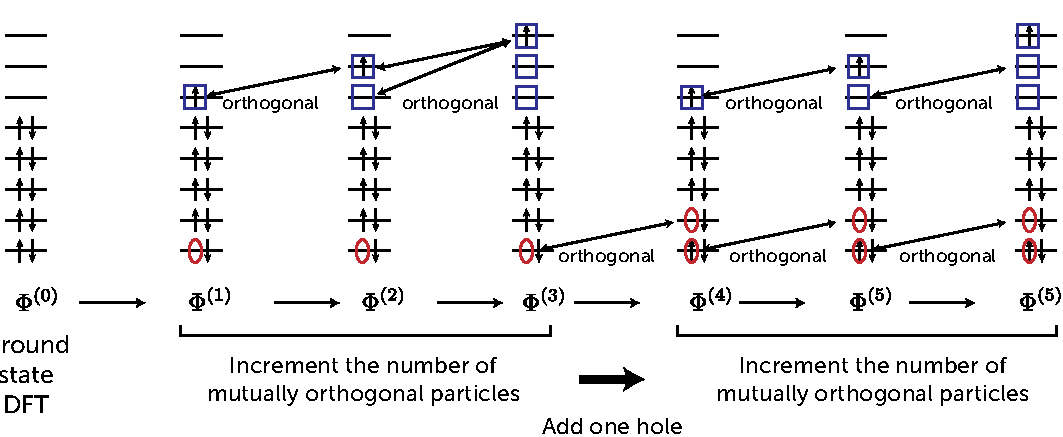
\includegraphics[width=16cm]{Figure2.pdf}
\caption{Visual representation of the space spanned by all projection operators for the ground state determinant $|\Phi\rangle$ and the excited state determinant $|\Phi^{(1)}\rangle$. Notice that the hole orbital comes from the space spanned by $\hat{P}$ and that the particle orbital comes from the space spanned by  $\hat{Q}$, this is a direct result of Equations 2 and 3.}
\label{fig:projection}
\end{figure*}

Thus, the conditions considered here \textit{preserve strict orthogonality among all states}, but are not equivalent to the \textit{minimum} orthogonality conditions.

  For example, we require that for state $\Phi_n$ at least one orbital ${\phi^{(n)}_j}$ is orthogonal to the occupied orbitals of all lower states $\Phi_m$ ($m < n$):
\begin{align}
\braket[1]{\phi^{(m)}_i}{\phi^{(n)}_{\rm p}} &= 0 \;\;\; \forall i \\
\braket[1]{\phi^{(m)}_a}{\phi^{(n)}_{\rm h}} &= 0 \;\;\; \forall a
\end{align}

a different approach that imposes exact orthogonality but relaxes the requirement of 


How do we generalize this to multiple excitations? \\
Dipole moments?\\
How do we compute contribution of various orbitals.



It is possible to extend this formulation to multiple excited states by simply removing the hole belonging to the previous excited state from the spectator space
\begin{align}
%\notag (1-\hat{Q}) (1 - \hat{Q}_s)\hat{f} |\phi_{\text{h}}^{\text{(1)}}\rangle &= \epsilon^{\text{(1)}}_{\text{h}} |\phi_{\text{h}}^{\text{(1)}}\rangle \\
%\notag (1-\hat{Q}) (1 - \hat{Q}_s - (\hat{P}^{(1)}_{\text{h}}))\hat{f} |\phi_{\text{h}}^{\text{(2)}}\rangle &= \epsilon^{\text{(2)}}_{\text{h}} |\phi_{\text{h}}^{\text{(2)}}\rangle \\ 
%\notag (1-\hat{Q}) (1 - \hat{Q}_s - (\hat{P}^{(1)}_{\text{h}} + \hat{P}^{(2)}_{\text{h}}))\hat{f} |\phi_{\text{h}}^{\text{(3)}}\rangle &= \epsilon^{\text{(3)}}_{\text{h}} |\phi_{\text{h}}^{\text{(3)}}\rangle\\
%\notag \vdots\\
\hat{P}[1 - \hat{Q}_s - (\hat{P}^{(1)}_{\text{h}} + \hat{P}^{(2)}_{\text{h}} + ... +\hat{P}^{\text{(k-1)}}_{\text{h}})]\hat{f} |\phi_{\text{h}}^{\text{(k)}}\rangle &= \epsilon^{\text{(k)}}_{\text{h}} |\phi_{\text{h}}^{\text{(k)}}\rangle .
\end{align}
Using this method extends the CH algorithm to allow the calculation of any excited state ``$k$''. We refer to this as the multi-constrained hole projection (MCHP) algorithm. It is important to note here that the ordering of the energy eigenvalues is not arbitrary, they are ordered by increasing orbital energy
\begin{align}
\epsilon^{\text{(1)}}_{\text{h}} \le \epsilon^{\text{(2)}}_{\text{h}} \le \epsilon^{\text{(3)}}_{\text{h}} \le ... \le \epsilon^{\text{(k)}}_{\text{h}} .
\end{align}
Because of this, in order for the MCHP algorithm to obtain the energy for the $k^{\text{th}}$ excited state, it must first project out all holes related to excited states 1 $\rightarrow$ $(k-1)$.

\begin{figure}
\centering
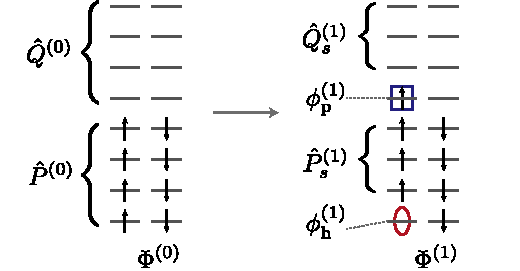
\includegraphics[width=8.8cm]{Figure1.pdf}
\caption{Visual representation of the space spanned by all projection operators for the ground state determinant $|\Phi\rangle$ and the excited state determinant $|\Phi^{(1)}\rangle$. Notice that the hole orbital comes from the space spanned by $\hat{P}$ and that the particle orbital comes from the space spanned by  $\hat{Q}$, this is a direct result of Equations 2 and 3.}
\label{fig:projection}
\end{figure}

\section{Computational Details}
Our OCDFT for core-excited states was implemented as a plugin for the \textsc{psi4} \textit{ab initio} quantum chemistry package.\cite{turney_psi4:_2012} The OCDFT excitation energies reported in this study were computed using the B3LYP, \cite{becke_new_1993,lee_development_1988,vosko_accurate_1980,stephens_ab_1994} PBE0 \cite{adamo_toward_1999}, and BLYP\cite{stephens_ab_1994,miehlich_results_1989} functionals, using the correlation-consistent polarized core-valence basis sets (cc-pCV$X$Z, $X$ = T,Q)\cite{woon_gaussian_1995-1}
and the Karlsruhe valence polarized basis sets (def2-$X$ZVP, $X$ = T,Q).\cite{weigend_balanced_2005,weigend_accurate_2006} All geometries were optimized at the same level of theory as the given excitation energy.
TDDFT calculations were performed at the B3LYP level of theory with the def2-TZVP basis set for the sake of comparison. All TDDFT calculations were performed with the ORCA software package\cite{neese_orca_2012}.

It is mandatory to consider relativistic effects when studying excitations of core electrons.\cite{maganas_l-edge_2014,debeer_george_calibration_2010,bauer_herfd-xas_2014,ankudinov_sensitivity_2002}
%Work by Desclaux et al. \cite{desclaux_relativistic_1971} shows that the largest orbital effect when solving the relativistic hartree-fock equations is the contraction of the 1s orbital, the corresponding energy correction ($\Delta\epsilon_{\text{1s}}$) can be approximated by 
For excitations involving 1s orbitals, we approximate the relativistic excitation energy ($\omega^{\rm R}$) as the sum of the nonrelativistic excitation energy ($ \omega^{\rm NR}$) minus a correction $\Delta\epsilon_{\text{1s}}$:
\begin{align}
\omega^{\rm R} = \omega^{\rm NR} - \Delta\epsilon_{\text{1s}} ,
\end{align}
where $\Delta\epsilon_{\text{1s}}$ is the energy difference between the ground-state nonrelativistic (NR) and relativistic (R) Kohn--Sham energies of the 1s orbital:
\begin{align}
\Delta\epsilon_{\text{1s}} = \epsilon_{\text{1s}}^{\text{R}} - \epsilon_{\text{1s}}^{\text{NR}}.
\end{align}
In this work, the excitation energies computed in OCDFT and TDDFT utilize relativistic orbital energies calculated with first-order Douglass--Kroll--Hess (DKH) Hamiltonian.\cite{douglas_quantum_1973,hess_applicability_1985, hess_relativistic_1986} 
Relativistic corrections for the 1s orbitals of the second row nuclei range from 3.8 eV (Si) to 10.1 eV (Cl). 
In the case of first row 1s core orbitals, $\Delta\epsilon_{\text{1s}}$ is negligible (C, N, and O 1s corrections are about 0.1, 0.2, and 0.3 eV, respectively).  Similarly, excitations from 2p orbitals of second row elements are negligible (max 0.05 eV) and were not applied to the final results.

The treatment of core-excited states in molecules with symmetry equivalent atoms becomes problematic for both pure and hybrid functionals due to the approximate treatment of exchange and correlation which introduces a self-interaction error.\cite{bally_incorrect_1997,lundberg_quantifying_2005} In this case, the symmetry restricted solution produces core holes distributed evenly amongst the symmetry equivalent atoms. 
Instead, the symmetry unrestricted solution may consists of core holes localized on  each individual atom. 
For all molecules with symmetry equivalent atoms (N$_2$, C$_2$H$_2$, and Cl$_2$) we studied both the symmetry restricted and unrestricted solutions.
To obtain a state where the core hole is localized, we utilize a wavefunction with broken spatial and spin symmetry mixing the coefficients of the alpha and beta orbitals.
\\
The optimized geometries and the NEXAS spectra of adenine and thymine were computed at the def2-TZVP/B3LYP level of theory. Peak intensities were approximated by taking the transition dipole moments ($\mu_i$) and calculating an oscillator strength ($f_{\rm osc} $) for each transition ($\omega_{i}$)
  \begin{align}
  \label{osc}
  f_{\rm osc} = \frac{2}{3} (\mu_x^2 + \mu_y^2 + \mu_z^2) \omega_{i}
  \end{align}
Eq. \eqref{osc} yields the absolute oscillator strength ($f_{\rm abs}$) for a given transition. The intensity of the spectra is then scaled relative to the most intense peak, we will refer to these scaled values as the \textit{relative oscillator strength} ($f_{\rm rel}$). The peaks are represented by convoluted gaussians centered around the frequency of each calculated transition, each gaussian has a FWHM between 0.1 - 0.4 eV (corresponding to the best fit to the experimental spectra) in order to simulate natural spectroscopic broadening effects. 

\section{Results and Discussion}
%OCDFT was used to compute 40 unique core-excitations from a test set of 13 molecules. Its accuracy was assessed by comparing it to experimental data from gas-phase NEXAS experiments.\cite{puttner_vibrationally_1999,remmers_high-resolution_1992,chen_k-shell_1989,tronc_nitrogen_1980,tronc_carbon_1979,francis_studies_1994,adachi_vibronic_1999,hitchcock_k-shell_1979,domke_carbon_1990,nayandin_angle-resolved_2001,bodeur_single-and_1990} 
%Excitations from 1s orbitals are considered for all multi-electron atoms in each molecule, in addition to excitations from 2p orbitals for second row elements. 
%The MAEs of OCDFT over the test set are shown in Table \ref{table:OverallPerformance}, considering 12 unique basis set and functional combinations. A direct comparison of the accuracy of OCDFT and TDDFT compared to experimental core-excitation energies are shown in Figure \ref{figure:Hist}. A breakdown of individual excitations computed with OCDFT and TDDFT are compared to their experimental assignments in Tables \ref{table:FirstRow} and \ref{table:SecondRow}. Table \ref{table:FirstRow} displays excitations from first row atoms, while Table \ref{table:SecondRow} shows excitations from second row atoms. We observe a distinct relationship between the amount of hole/particle orbital overlap and the accuracy of the computations, this relationship is explained in Section 4.3 and further analyzed in Figure \ref{figure:scatter}. Finally we close by computing the NEXAS spectra of two nucleobases, adenine and thymine. The nitrgen, carbon, and oxygen edges for Thymine can be found in Figure \ref{figure:Thymine} while the carbon and nitrogen edges of Adenine are found in Figure \ref{figure:Adenine}. Spectra resulting from inner-shell ionizations are commonly referred to as K, L, or M edges depending on which core-shell is involved in the excitation. This nomenclature is simply derived from the Barkla labeling scheme for X-ray series, and we will routinely employ it to refer to specific spectra.
\indent The average error of OCDFT over the full test set of first and second row core excitations are shown in Table \ref{table:OverallPerformance}, considering 12 unique basis set and functional combinations.
%First we present evidence that OCDFT is an accurate method for the computation of core-excited states. This is proven by benchmarking OCDFT over a test set of 40 unique core excited states over 13 different molecules.
Our test set comprises molecules containing first-row (CO, H$_2$CO, N$_2$O, N$_2$, HCN, CH$_4$, C$_2$H$_4$) and second-row elements (SiH$_4$, PH$_3$, H$_2$S, SO$_2$, HCl, Cl$_2$). Individual excitation energies computed with OCDFT and TDDFT are compared to values from gas-phase NEXAS experiments \cite{puttner_vibrationally_1999,remmers_high-resolution_1992,chen_k-shell_1989,tronc_nitrogen_1980,tronc_carbon_1979,francis_studies_1994,adachi_vibronic_1999,hitchcock_k-shell_1979,domke_carbon_1990,nayandin_angle-resolved_2001,bodeur_single-and_1990} in Tables \ref{table:FirstRow} and \ref{table:SecondRow}. Table \ref{table:FirstRow} displays excitations from first row atoms, while Table \ref{table:SecondRow} shows excitations from second row atoms. \\ 
\indent The three functionals considered in Table \ref{table:OverallPerformance} produce MAEs ranging from 0.9 eV $\rightarrow$ 1.7 eV, exhibiting that there is no dramatic difference in the accuracy of OCDFT regardless of the amount of Hartree--Fock (HF) exchange present in the functional. Even the BLYP functional, which contains no HF exchange, yields a MAE of 1.0 eV $\rightarrow$ 1.5 eV, which is comparable to the MAEs produced by it's hybrid counterparts. B3LYP produces errors in the range of 1.0 eV $\rightarrow$ 1.5 eV, while PBE0 produces errors in the range of 0.9 eV $\rightarrow$ 1.7 eV. BLYP outperforms PBE0 when employing three of the fours basis sets considered and yields similar MAEs as B3LYP. The Karlsruhe family of basis sets yields results that are in better agreement with the experimental excitation energies than the correlation consistent basis sets.
\begin{table}[!ht]
\small
\centering
    \begin{tabular}{lccc}
    \hline
    \hline
Basis Set & \multicolumn{3}{c}{Mean Absolute Error (eV)}  \\
& BLYP & B3LYP & PBE0\\
\hline
def2-TZVP & 1.0 & 1.0 & 0.9 \\
def2-QZVP & 1.0 & 1.0 & 1.4 \\
cc-pCVTZ & 1.3 & 1.3 & 1.6 \\
cc-pCVQZ & 1.5 & 1.5 & 1.7 \\
\hline
\hline
\end{tabular}
    \caption{Mean absolute error in the core-excited states calculated using OCDFT on a test set of 35 different core excited states from 13 different molecules.}
    \label{table:OverallPerformance}
\end{table}
\\
The average error of OCDFT is commensurate to that of wavefunction methods for core-excited states. For example, Asmuruf and Besley\cite{asmuruf_calculation_2008} reported an average error of 1.2 eV for SOS-CIS(D) applied to a set of excitations similar to the ones used in the present study. While Coriani et al.\cite{coriani_coupled-cluster_2012} reported errors of less than 0.9 eV when applying coupled cluster response theory to a set of carbon, nitrogen, and neon core excitations. 
\\
A full comparison of the accuracy of OCDFT and TDDFT core-excitations computed at the B3LYP/def2-TZVP level of theory are shown in Fig. \ref{figure:Hist}. OCDFT performs very well,  yielding an error distribution peaked near zero and a maximum error of $-$3.7 eV. On the contrary, TDDFT performs rather poorly, underestimating the excitation energies, on average, by 15 eV with a maximum error of $-$53.6 eV. A common source of error in the calculation of core excited states is the inadequate treatment of relativistic effects. It is crucial that we reiterate that all excitation energies were computed using the DKH relativistic Hamiltonian, thus the underestimation of the excitation energies by TDDFT is not solely a product of relativistic effects.\cite{saue_relativistic_2011}
\begin{figure}[!ht]
\centering
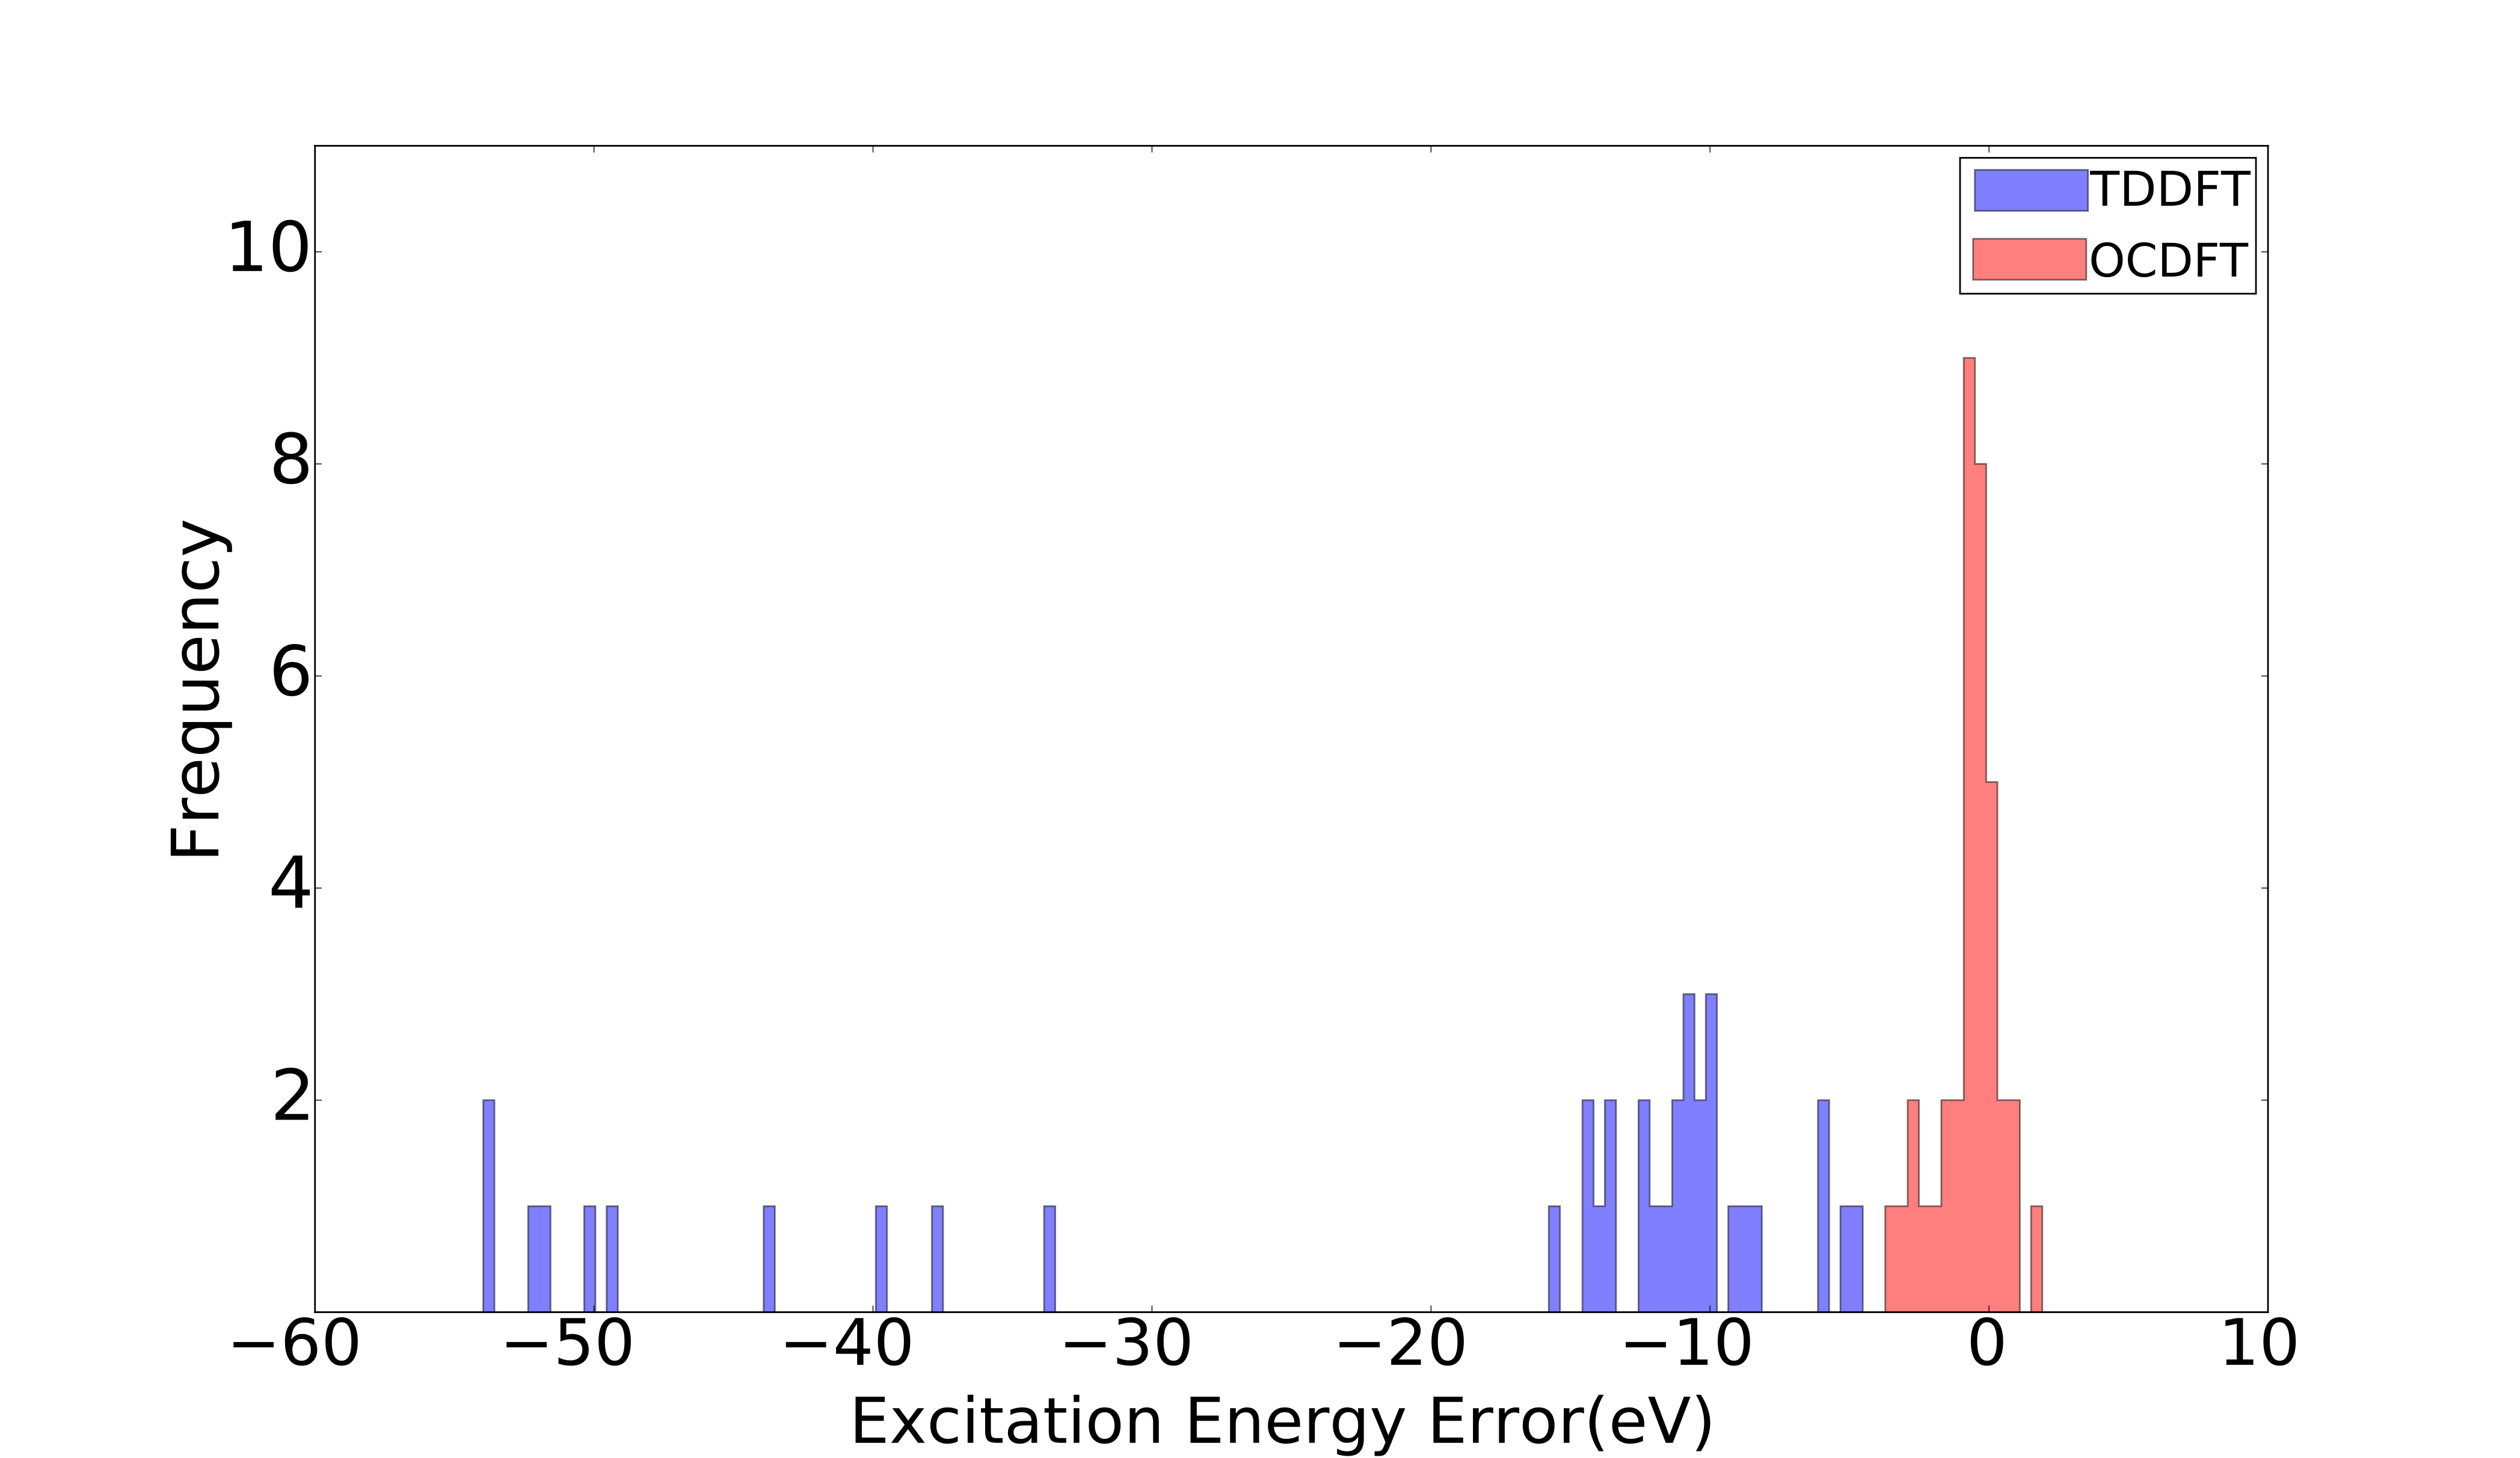
\includegraphics[width=8.8cm]{NEW_histogram.png}
\caption{Histogram showing the distribution of the error in the computed core excited states. All calculations were done using the B3LYP functional and the def2-QZVP basis set. The red filled bar is OCDFT while the empty blue bar is TDDFT.}
\label{figure:Hist}
\end{figure}
\\ \\
Fig. \ref{figure:Hist} hints at a specific difficulty of conventional TDDFT. Notice the gap, roughly 15 eV wide, that exists between the two clusters of TDDFT data. This gap exists because TDDFT becomes sharply more inaccurate when dealing with second row core excitations \cite{nakata_extension_2007,besley_time-dependent_2009}. 
%All of the TDDFT excitation energies that have an absolute error greater than 20 eV can be attributed to core excitations involving 1s orbitals located on second row nuclei. 
This dramatic difference in accuracy suggests that it is helpful to separately analyze first row and second row core excitations to highlight the distinctive challenges that arise in each case.
\noindent Table \ref{table:FirstRow} reports valence and Rydberg excitation energies of 1s orbital localized on first row elements (C, N, or O). TDDFT produces a mean absolute error of 11.6 eV compared to experiment, and as discussed earlier, this result is consistent with previous studies that used TDDFT with conventional hybrid functionals,\cite{besley_self-consistent-field_2009} OCDFT calculations yield a mean absolute error of 0.4 eV. To put this error into perspective, it can be compared to the performance of TDDFT with the BH$^{0.58}$LYP functional,\cite{besley_time-dependent_2009} a reparameterization of the BHLYP functional that has been augmented to include 58\% HF exchange, 39\% B88 exchange, and 8\% Slater exchange. When applied to a test set of first row core excitations similar to those in Figure \ref{table:FirstRow}, BH$^{0.58}$LYP yielded a mean average error of 0.8 eVs. A comparable level of accuracy was achieved by OCDFT without altering the inherent amount of HF exchange present in the functional. It is also gratifying to see that the OCDFT MAE for this set of first row core excited states is comparable to the MAE obtained for valence excited states (0.3 eV reported in Ref. \citenum{evangelista_orthogonality_2013})
\\ \\ 
\begin{table}[!ht]
\small
    \centering
    \begin{tabular*}{8.8cm}{lllllHH}
    \hline
    \hline
     Molecule & Excitation                     & Exp. (eV) & \multicolumn{2}{c}{Error (eV)} \\ ~&~ &~   & TDDFT  & OCDFT\\
     \hline
    \multirow{4}{*}{CO}        & C 1s $\rightarrow$ $\pi^*$     & 287.4 & $-$11.3     & $-$0.8  & $-$10.9    & \ 0.9   \\
             & C 1s $\rightarrow$ 3s          & 292.4 & $-$10.5     & \ 0.9   & $-$10.8    & \ 1.2   \\
             & O 1s $\rightarrow$  $\pi^*$    & 534.2 & $-$13.4     & $-$1.2  & $-$14.4    & $-$1.4   \\
             & O 1s $\rightarrow$ 3s          & 538.9 & $-$13.0     & \ 0.2 \vspace{2mm}   & $-$13.9    & \ 0.3 \\ 
    \multirow{4}{*}{H$_2$CO }     & C 1s $\rightarrow$ $\pi^*$     & 286.0   & $-$10.7     & $-$0.6  & $-$10.7    & $-$0.8   \\
    ~         & C 1s $\rightarrow$ 3s          & 290.2 & $-$10.7     & $-$0.2   & $-$10.7    & $-$0.3   \\
    ~         & O 1s $\rightarrow$ 3s          & 535.4 & $-$14.1     & $-$0.6   & $-$14.1    & $-$0.7   \\
    ~         & O 1s $\rightarrow$  $\pi^*$    & 530.8 & $-$14.0    & $-$0.8 \vspace{2mm}   & $-$14.1    & $-$1.1  \\
    \multirow{6}{*}{N$_2$O$^{\dagger}$}    &O 1s  $\rightarrow$ $\pi^*$ &  534.8 & $-$14.3 &  $-$1.0 & $-$14.3 & $-$1.3 \\
    ~         &O 1s  $\rightarrow$ 3s &  536.7 & $-$13.6 &  $-$0.4 & $-$13.6 & $-$0.6 \\
    ~         & N$_\text{c}$ 1s $\rightarrow$ 3s      & 407.5 & $-$12.1     & \ 0.6   & $-$12.6    & \ 0.6   \\
    ~         & N$_\text{t}$ 1s $\rightarrow$ $\pi^*$ & 401.1 & $-$12.2     & $-$0.9  & $-$14.6    & \ 2.5   \\
    ~         & N$_\text{t}$ 1s $\rightarrow$ 3s      & 404.0   & $-$11.5    & $-$0.4  \vspace{2mm} & $-$11.0    & $-$0.5  \\
    \multirow{3}{*}{N$_2$}         &N 1s  $\rightarrow$ $\pi^*$ & 401.0 & $-$12.4 & $-$0.9 & $-$12.4 & $-$1.1 \\
    ~         & N 1s  $\rightarrow$ 3s & 406.2 & $-$8.5 & 1.7 \vspace{2mm} & $-$7.2 & \ 2.7\\ 
    \multirow{4}{*}{HCN}       & C 1s $\rightarrow$ $\pi^*$     & 286.4 & $-$10.6     & $-$0.5  & $-$10.6    & $-$0.7  \\
    ~         & C 1s $\rightarrow$ 3s          & 289.1 & $-$9.9      & $-$0.1   & $-$9.9    & $-$0.3  \\
    ~         & N 1s $\rightarrow$  $\pi^*$    & 399.7 & $-$12.0     & $-$0.8  & $-$12.0    & $-$1.0  \\
    ~         & N 1s $\rightarrow$ 3s          & 401.8 & $-$10.4      & \ 0.2 \vspace{2mm}   & $-$10.4    & \ 0.0  \\
    \multirow{2}{*}{CH$_4$}      & C 1s $\rightarrow$ 3p          & 288.0   & $-$10.1      & \ 0.1   & $-$10.1    & \ 0.0   \\
    ~         & C 1s $\rightarrow$ 3s          & 287.1 & $-$10.8    & $-$0.5 \vspace{2mm}  & $-$10.8     & $-$0.6 \\ 
        \multirow{2}{*}{C$_2$H$_2$}      & C 1s $\rightarrow$ $\pi^*$           & 285.8   & $-$10.5      & $-$0.1   & $-$10.4   & $-$0.7  \\
    ~         & C 1s $\rightarrow$ 3s            & 287.7 & $-$9.1 & $-$0.6 \vspace{2mm}  & $-$8.9    & $-$0.3 \\
    ~MAE         &                            & ~     & 11.6      & 0.4   & 11.7     & 0.6 \\ 
    \hline
    \hline
    \end{tabular*}
    \caption{Core excitation energies for molecules containing first-row elements. Computations were performed using the B3LYP density functional and def2-QZVP basis set. The OCDFT and TDDFT results are reported here as deviations from the experimental value in electron volts (eV), mean absolute error (MAE) is also reported for each method. \\
    $^{\dagger}$For N$_2$O the subscript c and t stand center and tail nitrogen respectively.}
     \label{table:FirstRow}
     \end{table}
\subsection{Importance of Orbital Overlap}
When computing core excited states of second row nuclei, TDDFT becomes highly inaccurate, producing in an average error larger than 30 eV, even when the DKH relativistic corrections are included. Previous work by Tozer and coworkers \cite{peach_excitation_2008}  showed that there is a correlation between the level of accuracy of TDDFT excitation energies and the amount of overlap between the orbitals involved. We expect this correlation to also be observed in core electron excitations, where the
\begin{figure}[ht]
\centering
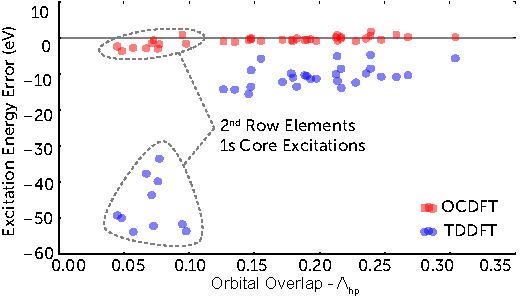
\includegraphics[width=8.8cm]{scatterNEWER2.pdf}
\caption{Scatterplot displaying the excitation energy error as a function of orbital overlap. Excitation energies were calculated using the B3LYP functional and def2-QZVP basis set. The overlap integrals were computed with numerical grid integration making use of the Gaussian cube files produced by in Psi4 OCDFT calculations. Grids were calculated with a double zeta basis set and 0.1 grid spacing.}
\label{figure:scatter}
\end{figure}
core hole and valence particle orbitals have little overlap. Following Tozer et al. ,\cite{peach_excitation_2008}we define the overlap between the hole and particle orbital ($\Lambda_{hp}$) for any excited state $n$ as the integral:
\begin{align}
\Lambda_{hp} = &\int |\phi^{(n)}_{\rm h} (\bf{r})||\phi^{(\textit{n})}_{\rm p} (\bf{r})| \ \rm d\bf{r} ,
\end{align}
where $\Lambda_{hp}$ ranges from 0 to 1. Figure \ref{figure:scatter} reports the distribution of excited states as a function of the error and the overlap in OCDFT and TDDFT. This highlights the effect that a decrease in orbital overlap has on the accuracy of the excitation energy computed with OCDFT and TDDFT. The vertical dashed line at 0.12 separates the low overlap region (containing exclusively excitations from second row 1s core orbitals) from the higher overlap region (containing exclusively excitations from first row 1s and second row 2p core orbitals). The scatterplot clearly shows that OCDFT is less sensitive to variations in the overlap. Transitioning from the low overlap region to the high overlap region the MAE increases by only 1.5 eV for OCDFT, while in the case of TDDFT the absolute error increases drastically by 35.9 eV.\\
\begin{table}[!ht]
\footnotesize
    \centering
    \begin{tabular*}{8.8cm}{lllllHH}
    \hline
    \hline
     Molecule & Excitation                     & Exp. (eV) & \multicolumn{2}{c}{Error (eV)} \\ ~&~ &~   & TDDFT  & OCDFT\\
     \hline
    \multirow{2}{*}{SiH$_4$}        & Si 1s $\rightarrow$ $\sigma^*$     & 1842.5 & $-$38.4    & $-$1.8  & $-$38.9    & $-$2.3   \\
             & Si 2p $\rightarrow$ $\sigma^*$ & 102.8 & $-$4.8 & 0.6 \vspace{2mm}   & $-$4.1    & 1.5 \\
    \multirow{2}{*}{PH$_3$ }     & P 1s $\rightarrow$ $\sigma^*$ & 2145.8   & $-$44.1     & $-$2.9  & $-$44.1    & $-$3.2   \\
    ~         & P 2p $\rightarrow$ $\sigma^*$          & 132.3 & $-$5.1     & 0.7  \vspace{2mm} & $-$5.1    & 0.0 \\
    \multirow{4}{*}{H$_2$S}    &S 1s  $\rightarrow$ $\sigma^*$ &  2473.1 & $-$48.3 &  $-$3.0 & $-$48.3 & $-$3.8 \\
    ~         &S 1s  $\rightarrow$ 4p &  2476.3 & $-$52.1 &  $-$1.5 & $-$52.1 & $-$0.6 \\
    ~         & S 2p $\rightarrow$ $\sigma^*$ & 164.5 & $-$5.1    & 0.8  & $-$5.1    & 0.4  \\
    ~         & S 2p $\rightarrow$ 4s      & 166.5 &  $-$7.1    & $-$0.7 \vspace{2mm}   & $-$7.1    & $-$1.0 \\
    \multirow{3}{*}{SO$_2$}         &S 1s  $\rightarrow$ $\pi^*$ & 2473.8 & $-$50.1 & $-$3.7 & $-$51.3 & $-$4.5 \\
    ~         & S 1s  $\rightarrow$ 4p & 2478.4 & $-$49.3 & $-$2.4 & $-$50.4 & $-$3.2 \\
    ~         & S 2p $\rightarrow$ 4s      & 171.3 & $-$8.3     & $-$1.5 \vspace{2mm}   & $-$8.2    & $-$1.9 \\
    \multirow{3}{*}{HCl}       & Cl 1s $\rightarrow$ $\sigma^*$     & 2823.9 & $-$53.8     & $-$2.3  & $-$55.4    & $-$4.7  \\
    ~         & Cl 1s $\rightarrow$ 4p          & 2827.8 & $-$52.1      & $-$0.7   & $-$52.7    & $-$1.7  \\
    ~         & Cl 2p $\rightarrow$  $\sigma^*$    & 201.0 & $-$6.1 & 0.8 \vspace{2mm}  & $-$6.1    & 0.3 \\
    \multirow{3}{*}{Cl$_2$}      & Cl 1s $\rightarrow$ $\sigma^*$          & 2821.3   & $-$53.6      & $-$1.6   & $-$55.3    & $-$3.6   \\
    ~         & Cl 1s $\rightarrow$ 4p          & 2828.5 & $-$51.7    & 0.9  & $-$53.5     & $-$0.2  \\
        ~         & Cl 2p $\rightarrow$  $\sigma^*$    & 198.7 & $-$5.7     & $-$0.8 \vspace{2mm} & $-$5.8    & $-$0.3\\
    MAE         &                            & ~     & 31.6      & 1.6   & 32.0     & 2.0   \\
    \hline
    \hline
    \end{tabular*}
    \caption{Calculated core excitation energies for excitations involving 1s/2p electrons of second-row atoms. Computations were performed using the B3LYP density functional and def2-QZVP basis set, the values reported here are the deviations from the experimental value in electron volts (eV). Mean Absolute Error (MAE) is reported for each method.}
     \label{table:SecondRow}
\end{table}
\begin{comment}
Multiple studies have concluded that the shortcoming of traditional density functionals is not the treatment of long-range interaction, but instead it is the incorrect description of the core region that leads to inaccuracy. [CITE] This problem was specifically addressed by the SRC-BLYP functional \cite{besley_time-dependent_2009} which is a flexible functional that increases the amount of Hartree-Fock exchange at short range and is identical to the long range corrected CAM-BLYP at long range. 
\end{comment}

It has been concluded that varying HF exchange parameters can vastly improve the description of core-excited states,\cite{nakata_time-dependent_2006} however, here we approached the problem in a different way. With a slight augmentation to DFT derived from first principles, an accurate description of core excited states is possible without relying on varying the amount of HF exchange. \\
To understand why OCDFT outperforms TDDFT, we will consider a model consisting of one electron in two orbitals ($\phi_{\rm h}$, $\phi_{\rm p}$) and compare the TDDFT and OCDFT excitation energies to that of CIS, since, in this case, CIS is exact. Similar analyses have been reported for variational DFT \cite{ziegler_implementation_2012} and TDDFT. \cite{casida_charge-transfer_2000} For a functional containing a given fraction ($a$) of HF exchange, TDDFT and CIS excitation energies for our one electron model differ approximately by:
\begin{align}
\label{eq:TDDFT_CIS}
 \nonumber \omega^{\text{TDDFT}}_s - \ \omega^{\text{CIS}}_s &\cong (1 - a) [J_{\text{ph}} - J_{\text{hh}}] \\ &+ (1 - a) [\nu_{\text{p}}^x - \nu_{\text{h}}^x] ,
\end{align}
where $\nu_{\rm h}^x$ and $\nu_{\rm p}^x$ are the exchange potentials [$\nu_{\rm h/p}^x = (\phi_{\rm h/p}|\nu_x|\phi_{\rm h/p})$] for orbitals p and h, respectively. When $a \neq 1$, the term in Eq. ~\ref{eq:TDDFT_CIS} contains three local integrals $\nu_{\rm h}^x$, $\nu_{\rm p}^x$, and $J_{\text{hh}}$. However, the coulomb repulsion integral between the hole and particle orbitals ($J_{\text{ph}}$) is nonlocal and causes TDDFT to incorrectly describe charge transfer excitations. This nonlocality hampers TDDFT's treatment of core excitations as well. The improved performance of OCDFT for core excited states can be understood by investigating the local nature of the integrals involved. The excitation energy for OCDFT differs from CIS by a term that is composed of integrals that are localized on either the hole or the particle, which allows for a better approximation of core excited states in which the overlap of $\phi_{\rm h}$ and $\phi_{\rm p}$ is small.
\begin{align}
\nonumber \omega^{\text{OCDFT}}_s - \ \omega^{\text{CIS}}_s  &\cong (1 - a) [\nu_{\text{p}}^x - \nu_{\text{h}}^x + \frac{1}{2} J_{\text{pp}} - \frac{1}{2} J_{\text{hh}} \\
&+ \frac{1}{2} (\text{hh}|\hat{f}_x|\text{hh}) +\frac{1}{2} (\text{pp}|\hat{f}_x|\text{pp})] ,
\end{align}
where (ii$|\hat{f}_x|$ii) = $\int |\phi_{\text{i}}|^2\ \hat{f}_x\  |\phi_{\text{i}}|^2 \ d\tau$ are the exchange kernel integrals. The local nature of the integrals in this term provide a better approximation to exact exchange. This is a direct consequence of the orthogonality condition imposed between the ground and excited states, resulting in a term that is much more adept at handling systems with low orbital overlap.
\subsection{Application to Nucleobases: Thymine and Adenine Near-Edge Spectra}
\begin{figure}[!ht]
\centering
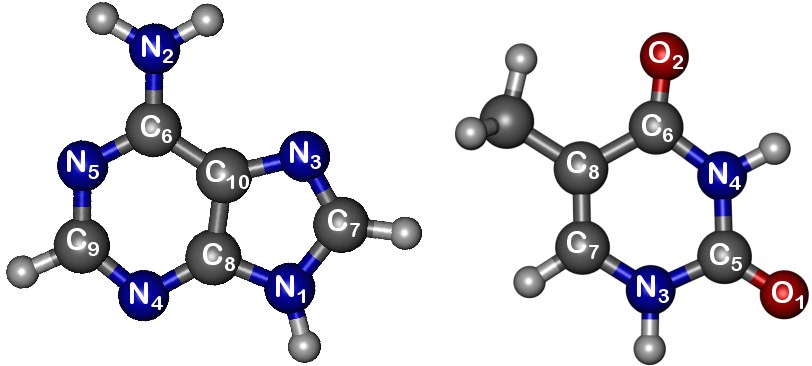
\includegraphics[width=8.8cm]{adenineThymineNumbering3D.png}
\caption{Numbering scheme of adenine (left) and thymine(right), atoms are assigned a number based on decreasing Hartree-Fock orbital energy of their 1s core orbital. }
\end{figure}
\begin{figure*}
\centering
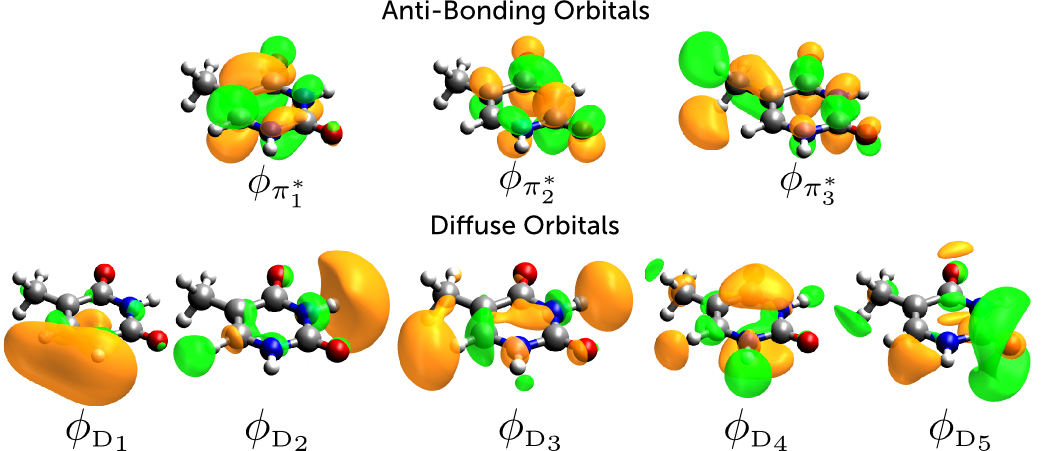
\includegraphics[width=14cm]{ThymineVirtuals.png}
\caption{Relevant virtual orbitals for thymine numbered in order based on orbital energy. Orbitals with obvious $\pi^*$ character are labeled as such, while orbitals where electron density is mostly diffused on the outside of the molecule are labeled as $\phi_D$.}
\end{figure*}
  Nucleobases are vastly important molecules that play a key biological role as the building blocks of DNA and recently show promise as potential materials for electronic/technological applications [CITE]. Early X-ray experiments on nucleobases were largely scattering and diffraction based techniques[CITE], it wasn't until 1992 that the first near-edge absorption experiments were performed by Mitra-Kirtley et al.\cite{kirtley_nitrogen_1992} In this study they selectively characterized the nitrogen environment and revealed the useful sensitivity of the 1s $\rightarrow$ $\pi^*$ resonances to the surrounding chemical environment. Modern experiments have moved beyond simple characterization and aim to probe interactions with surfaces and other applications. [CITE]  A wide array of computational methods have been used to compute the near-edge structure of these molecules, including: restricted active space SCF (RASSCF),\cite{mochizuki_hf-stex_2001} improved virtual orbital SCF (IVO-SCF)[CITE], a complex polarization propagator method (CPP) [CITE], SIC-DFT,\cite{bolognesi_investigation_2009} $\Delta$MP2,\cite{shim_calibration_2011} equivalent core approximation (ECA) method[CITE], and algebraic diagrammatic construction [ADC(2)][CITE]. \\
Here we present an OCDFT simulation of the thymine and adenine NEXAS spectra. We will first present the reader with an overview the performance of OCDFT relative to the classified peak maxima from gas-phase NEXAS experiments done by Plekan et al. [CITE] on both molecules. This will be followed by an in-depth analysis of the spectral features simulated in OCDFT to see how well they match the experimental spectra, and which excitations contribute to each feature. Then we will compare our work to previous theoretical work done at the ADC(2) level of theory. \\
\subsubsection{Overall Performance}
\ The simulation of the thymine and adenine NEXAS spectra shown in Figs.\ref{figure:Thymine} and \ref{figure:Adenine} agree well with the experimental data. A common feature of NEXAS spectra is the appearance of multiple low-intensity transitions that appear in the higher energy regions. This is represented well by OCDFT as evidenced by the stick spectra shown in Figs. \ref{figure:Thymine} and \ref{figure:Adenine} where the higher energy regions are populated by multiple low intensity transitions. Tables \ref{table: thymine_k_oxygen} - \ref{table: adenine_k_carbon} showcase the computed OCDFT excitations, with their corresponding 1s hole orbital ($\phi_h$), particle orbital ($\phi_p$), and relative oscillator strengths. Each transition can be interpreted as an excitation from $\phi_h$ $\rightarrow$ $\phi_p$. The experimental energies reported are the peak maxima for each spectral feature, and can be approximated by the OCDFT transition in that region with the strongest oscillator strength. When using this as a comparison, OCDFT represents the thymine peak maxima with an average error of 0.3 eV, and that of adenine with an average error of 0.1 eV. We emphasize that the computed OCDFT spectra are obtained from unshifted excitation energies. 
  \begin{figure}[!ht]
\centering
%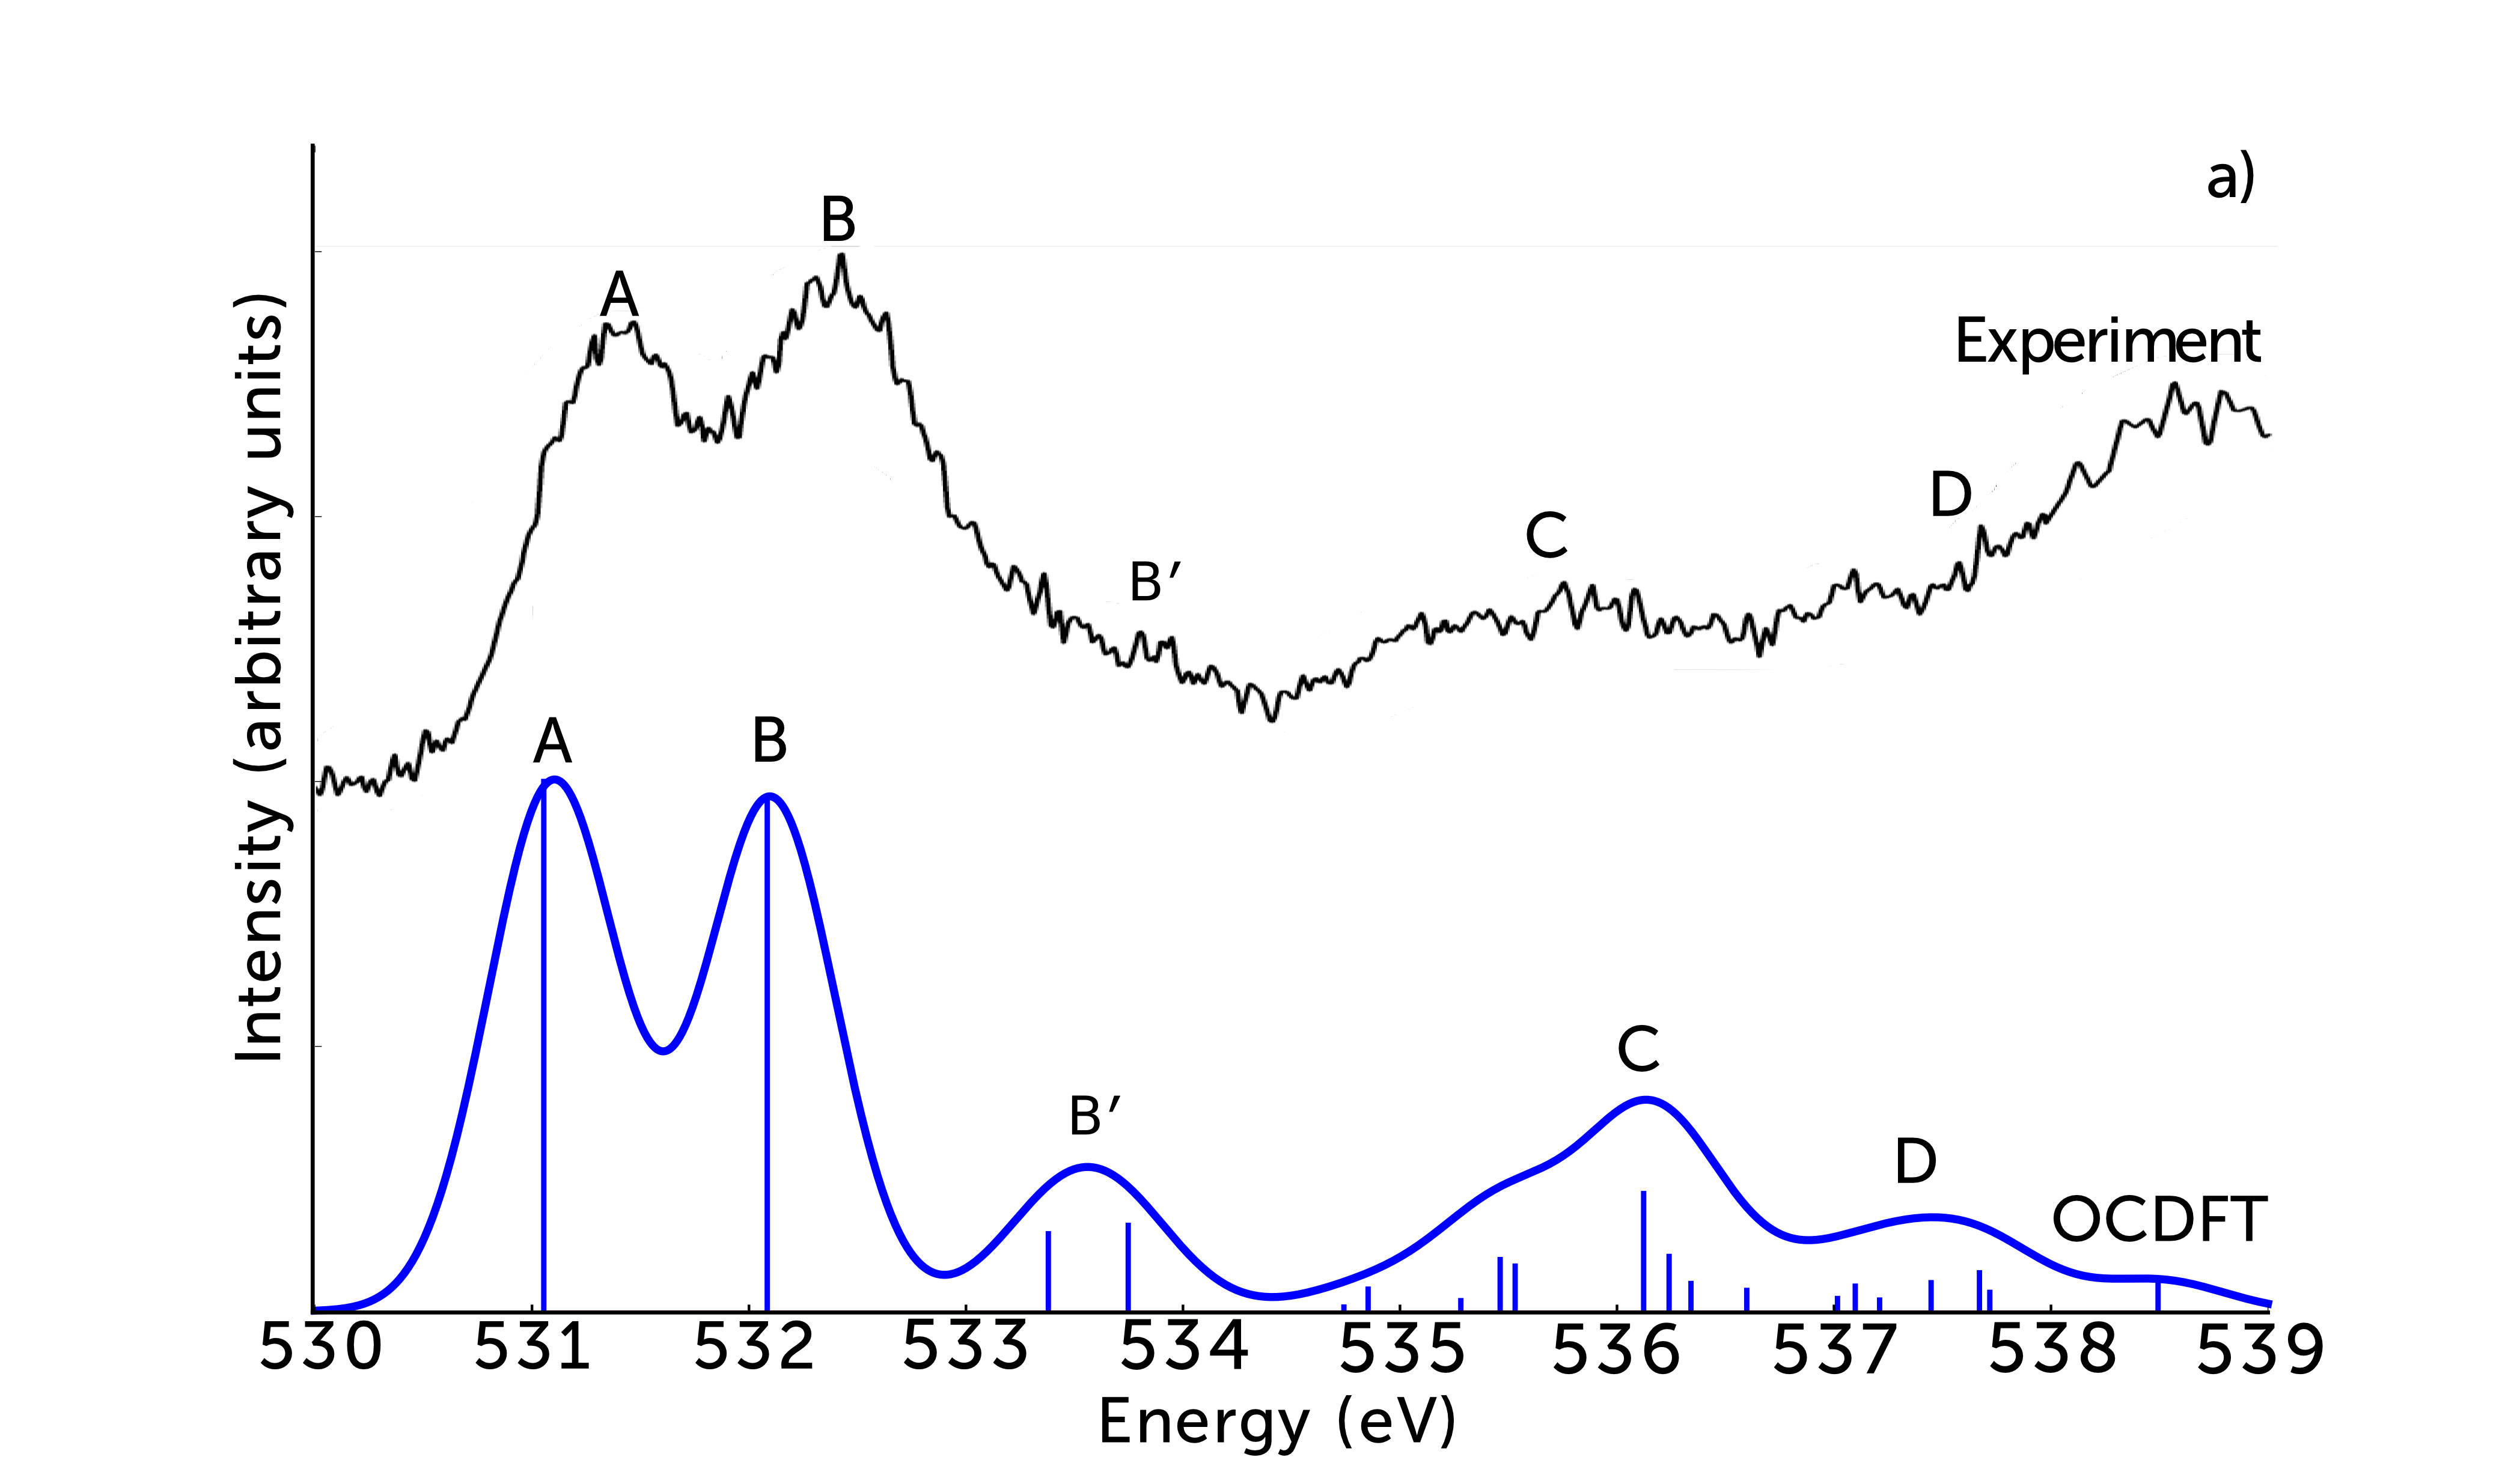
\includegraphics[width=8.8cm]{ThymineOKexperiment.png}\\
%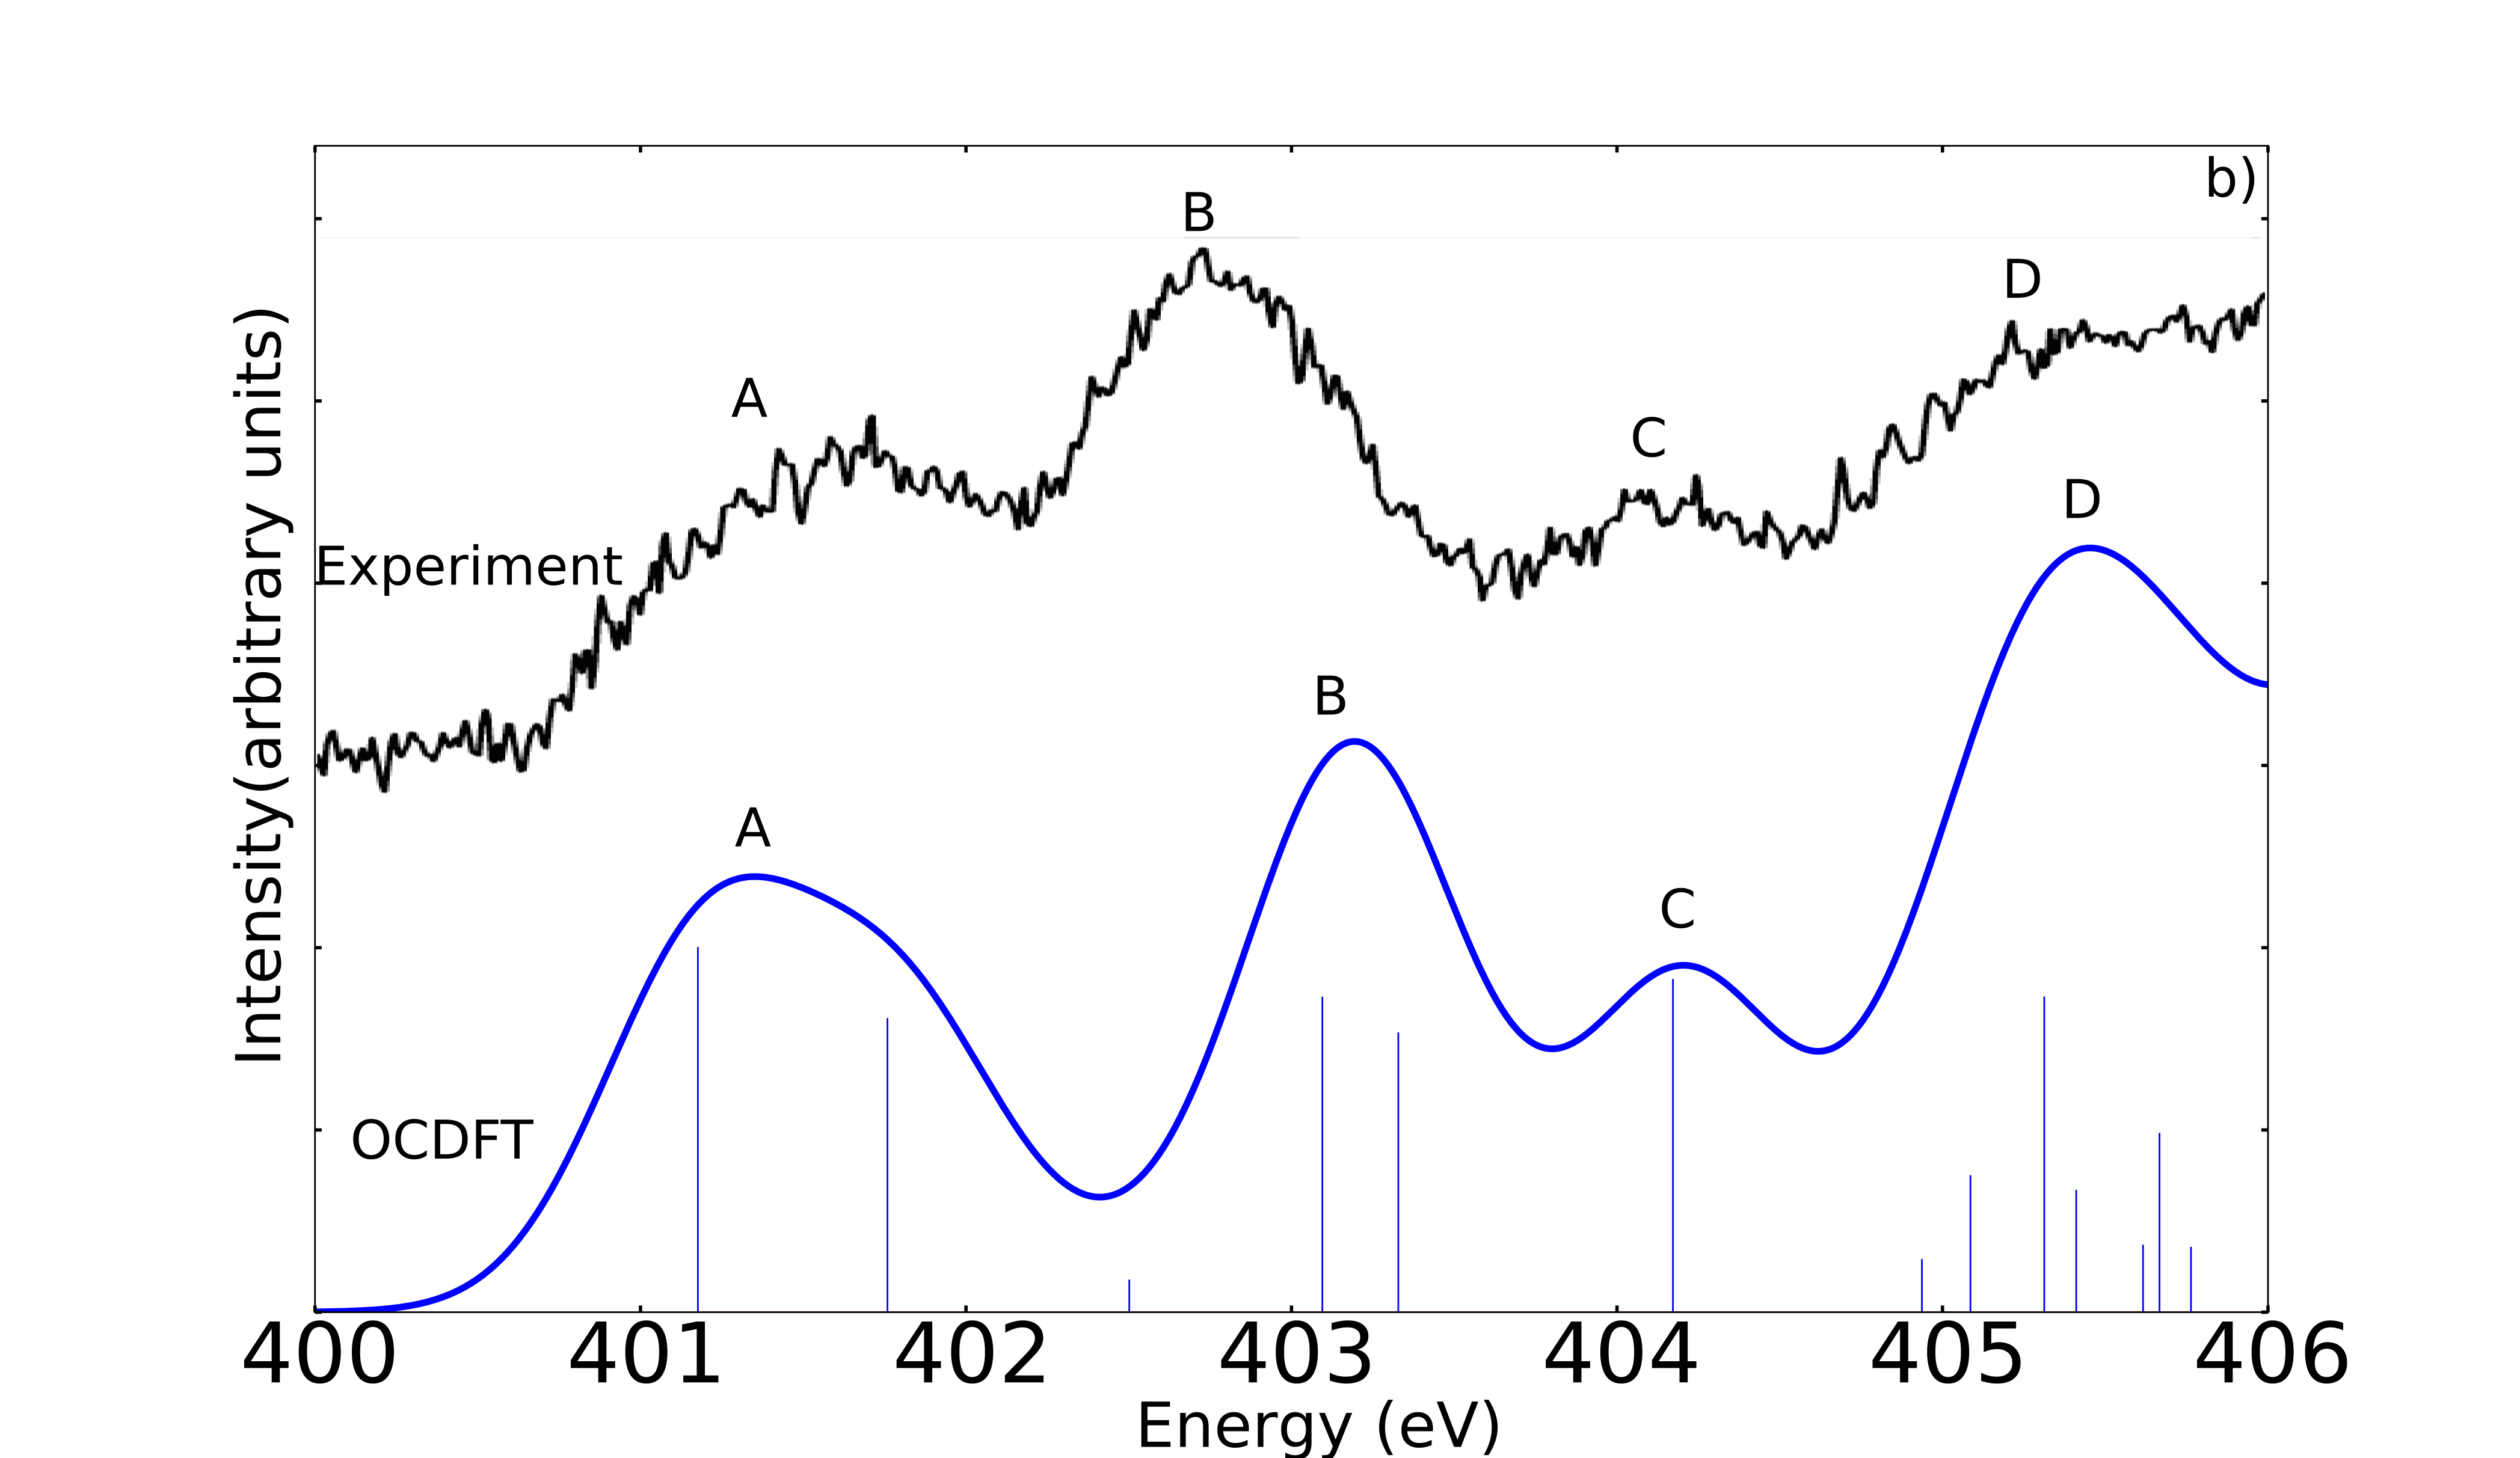
\includegraphics[width=8.8cm]{ThymineNKexperiment.png} \\
%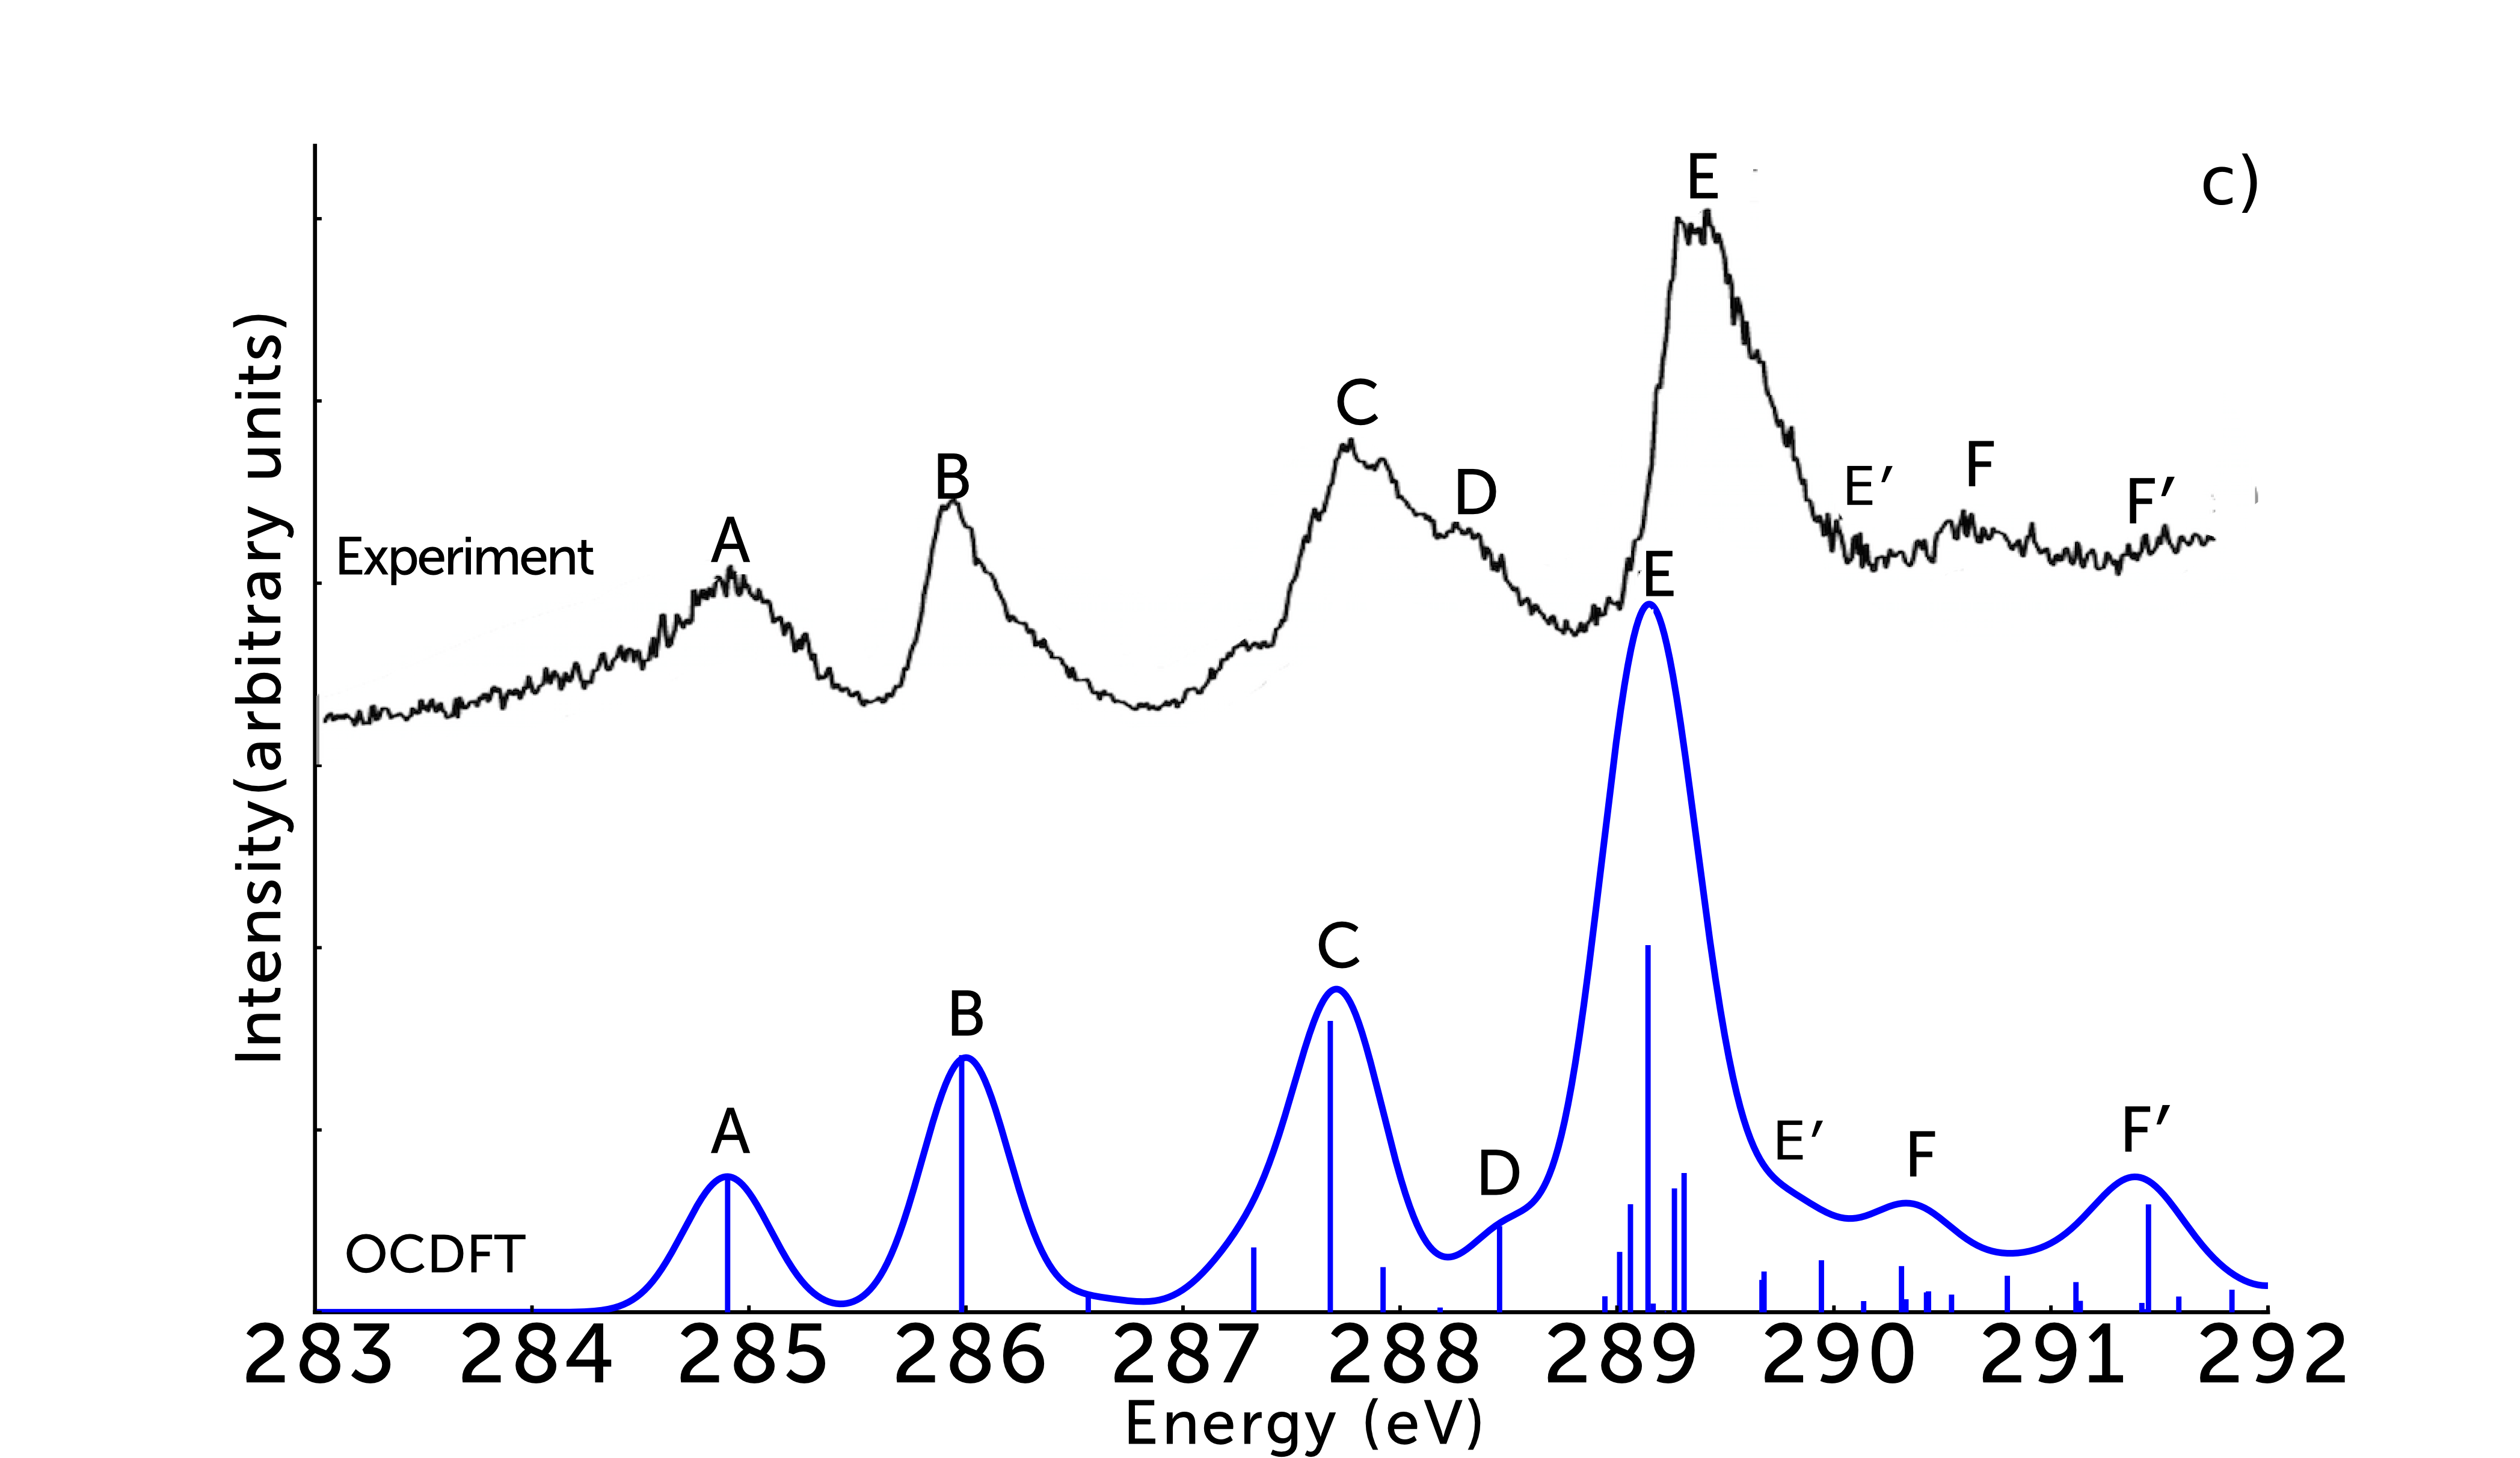
\includegraphics[width=8.8cm]{ThymineCKexperiment.png}
\caption{Core excited states for thymine computed using B3LYP functional and def2-TZVP basis set. Spectra is composed of convoluted Gaussians with a Full Width at Half Maximum (FWHM) of 0.3 eVs of the (a) oxygen K-edge (FWHM = 0.3 eV), (b) nitrogen K-edge (FWHM = 0.3 eV), and (c) carbon K-edge (FWHM = 0.2 eV). Experimental spectra is from reference [CITE].}
\label{figure:Thymine}
\end{figure}
\subsubsection{Thymine Oxygen K-Edge}
\ Figure \ref{figure:Thymine}a displays the experimental and theoretical spectra of thymine at the oxygen K-edge. The low energy regime of the oxygen K-edge is dominated by two high intensity peaks, Peak A results from the transition O$_2$ $\rightarrow$ $\pi^*_2$, while Peak B results from the transition O$_1$ $\rightarrow$ $\pi^*_1$ with a peak intensity that is roughly equal to that of Peak A. Experimentally, Peaks A and B are centered at 531.4 eV and 532.3 eV respectively, these excitation energies are predicted well by OCDFT to within 0.3 eV of the experimental peak assignments. The  O$_2$ $\rightarrow$ $\pi_2^*$ transition is predicted as the peak of highest intensity with an f$_{abs}$ of 0.02, these results are consistent with the ADC(2) analysis performed by Plekan et al (f$_{abs}$ = 0.03). The shoulder feature B$^{\prime}$ is composed of O$_1$ $\rightarrow$ $\pi^*_2$ and O$_2$ $\rightarrow$ $\pi^*_1$ and is predicted by OCDFT to have a fairly strong oscillator strength, this is inconsistent with the low intensity peaks that appear in this region in the experimental spectra.  As stated earlier, excitations of weaker intensity are characteristic of the higher energy regime of the K-Edge and have been attributed to strong mixing of core-valence excited states with Rydberg excited states of similar energy.[CITE] This strong mixing causes the character of each individual excitation to be spread out over several different final states, resulting in highly disordered peaks of weak intensity. The mixing in this region of the spectra makes it difficult to classify specific transitions experimentally. OCDFT results show that Peak C is largely composed of a mixture of 3s, 3p, and 4p Rydberg excitations within an energy interval of 534.7 to 536.4 eV. While the majority of the contributions to Peak D, are 4s and 4p excitations all with f$_{\text{rel}}$ $<$ 0.1. Peaks C and D both contain $\pi^*_3$ character, however the contributions from these resonances are weak and overshadowed by multiple Rydberg transitions in both cases. A small shoulder D$^{\prime}$ resulting from an excitation of O$_1$ $\rightarrow$ 5p is predicted by our method and is consistent with the tailing motif at the end of the spectra. \\
   \begin{table}
   \footnotesize
 \centering
     \begin{tabular}{c@{\hskip 0.22in}c@{\hskip 0.22in}c@{\hskip 0.22in}c@{\hskip 0.52in}c@{\hskip 0.22in}c@{\hskip 0.22in}c}
     \hline
     \hline
   \multicolumn{4}{c}{OCDFT} &\multicolumn{2}{c}{Experiment} \\
   \hline
 $\phi_h$ &  $\phi_p$ & $\omega_{fi}$ & f$_{rel}$ & Peak &  $\omega_{fi}$   \\
   \hline
    O$_2$
 &   81.8$\%$ $\pi_1^*$  & 531.05 & 1.000 & A  & 531.4 \vspace{0.05in}\\
    O$_1$
 &   64.0$\%$ $\pi_2^*$  & 532.08 & 0.968 & B & 532.3 \vspace{0.05in}\\
    O$_1$
 &   71.2$\%$ $\pi_1^*$  & 533.38 & 0.146 & \multirow{2}{*}{B$^{\prime}$} & \multirow{2}{*}{$\approx$ 533.8}  \\
    O$_2$
 &   78.3$\%$ $\pi_2^*$  & 533.75 & 0.162 \vspace{0.05in}\\
    O$_1$
 &   69.5$\%$ $\rm D_3$  & 535.46 & 0.098   & \multirow{3}{*}{C} & \multirow{3}{*}{535.7}  \\
    O$_1$
 &   76.0$\%$ $\pi_3^*$  & 536.12 & 0.222 \\
    O$_2$
 &   69.0$\%$ $\pi_3^*$  & 536.24 & 0.104 \vspace{0.05in}\\
    O$_1$
 &   83.5$\%$ $\rm D_4$  & 537.10 & 0.047 & \multirow{3}{*}{D} & \multirow{3}{*}{537.1} \\
    O$_1$
 &   35.6$\%$ 42-A  & 537.45 & 0.054 \\
    O$_2$
 &   44.0$\%$ 42-A  & 537.67 & 0.073 \\
\hline
\hline
   \end{tabular}
         \caption{Calculated and experimental thymine oxygen core excitation energies in eV are shown in the table. All computations are performed using the def2-TZVP basis set and B3LYP functional. The largest contribution to the particle orbital ($\phi_p$) with reference to the ground state valence set is reported along with the hole orbital ($\phi_h$) for each transition. Relative oscillator strengths (f$_{rel}$) are also reported}
   \label{table: thymine_k_oxygen}
   \end{table}
\subsubsection{Thymine Nitrogen K-Edge} \ The K-edge pictured in Figure \ref{figure:Thymine}b is characterized by four distinct spectral peaks. Unlike the oxygen spectra, the two lowest energy $\pi^*$ excitations merge into a single band (Peak A), rather than producing two distinct peaks. These lowest energy contributions to Peak A are excitations from N$_3$ and N$_4$ to $\pi^*_2$, OCDFT predicts their excitation energies to be 401.76 eV and 401.18 eV respectively. The experimental peak maximum is at 401.7 eV, which agrees well with the gaussian profile shown in the OCDFT spectra. Rydberg transitions from the N$_3$ and N$_4$ to 3s are the dominant resonances contributing to the character of peak B, along with a valence excitation N$_4$ $\rightarrow$ $\pi^*_1$ predicted at 402.50 eV. This agrees well with the experimental peak assignment at 402.7 eV. A very intense N$_4$ $\rightarrow$ 3p transition accounts for the peak at 404.1 eV, OCDFT simulates this peak perfectly with a gaussian centered at 404.17 eV. Peak D is the amalgamation of two $\pi^*$ resonances and multiple Rydberg states with the $\pi^*$ resonances being the transitions of strongest intensity. Excitation energies of these $\pi^*$ resonances agree well with the experimental peak assignment at 405.5 eV, with N$_4$ $\rightarrow$ $\pi^*_3$ at 405.31 eV and N$_3$ $\rightarrow$ $\pi^*_1$ at 405.66 eV.
  \\
      \begin{table}
     \footnotesize
 \centering
     \begin{tabular}{c@{\hskip 0.22in}c@{\hskip 0.22in}c@{\hskip 0.22in}c@{\hskip 0.52in}c@{\hskip 0.22in}c@{\hskip 0.22in}c}
     \hline
     \hline
   \multicolumn{4}{c}{OCDFT} &\multicolumn{2}{c}{Experiment} \\
   \hline
 $\phi_h$ &  $\phi_p$ & $\omega_{fi}$ & f$_{rel}$ & Peak &  $\omega_{fi}$   \\
   \hline
    N$_4$
 &   81.8$\%$ $\pi_1^*$  & 401.18 & 1.000 & \multirow{2}{*}{A} & \multirow{2}{*}{401.7} \\
    N$_3$
 &   64.0$\%$ $\pi_2^*$  & 401.76 & 0.805 
 \vspace{0.05in}\\
    N$_4$
 &   78.3$\%$ $\pi_2^*$  & 402.50 & 0.087 & \multirow{3}{*}{B} & \multirow{3}{*}{402.7}\\
    N$_3$
 &   77.0$\%$ $\rm D_1$  & 403.09 & 0.863 \\
    N$_4$
 &   65.9$\%$ $\rm D_1$  & 403.33 & 0.765 
 \vspace{0.05in}\\
    N$_4$
 &   44.1$\%$ $\rm D_3$  & 404.17 & 0.912 & C & 404.1 
 \vspace{0.05in}\\
    N$_3$
 &   69.5$\%$ $\rm D_3$  & 405.09 & 0.374  & \multirow{3}{*}{D} & \multirow{3}{*}{405.5} \\
    N$_4$
 &   86.3$\%$ $\rm D_4$  & 405.31 & 0.864 \\
    N$_3$
 &   71.2$\%$ $\pi_1^*$  & 405.67 & 0.490 \\
 \hline
 \hline
 \end{tabular}
  \caption{Calculated and experimental thymine nitrogen core excitation energies in eV are shown in the table. All computations are performed using the def2-TZVP basis set and B3LYP functional. The largest contribution to the particle orbital ($\phi_p$) with reference to the ground state valence set is reported along with the hole orbital ($\phi_h$) for each transition. Relative oscillator strengths (f$_{rel}$) are also reported}
   \label{table: thymine_k_nitrogen}
 \end{table}
\subsubsection{Thymine Carbon K-Edge} \
   The shape of the carbon K-edge displayed in Figure \ref{figure:Thymine}c is governed by four strong $\pi^*$ resonances. Unique to the carbon K-edge is the fact that the strongest transition is not the lowest energy $\pi^*$ resonance, the C$_5$ $\rightarrow$ $\pi_1^*$ transition is a relatively high energy excitation and produces the strongest peak intensity, despite close proximity to several Rydberg states. Peak A at 284.9 eV is the result of the transition C$_8$ $\rightarrow$ $\pi_2^*$, the position of this peak is predicted exactly by OCDFT. A slightly stronger transition at 285.9 eV is mostly due to a  C$_7$ $\rightarrow$ $\pi_2^*$ transition, with small contribution from another $pi_2^*$ resonance originating resulting from an excitation from the C$_9$ core. Peaks C and D have experimental peak maxima at 287.8 eV and 288.4 eV respectively, and blend together to form one band. Both contributions to the spectral band are represented well by OCDFT. The most prominent contributor to Peak C is the excitation from C$_6$ $\rightarrow$ $\pi^*_3$, while Peak D is the result of a C$_9$ $\rightarrow$ $\pi^*_3$. Peak E is mostly a fusion of Rydberg transitions, however these transitions have relatively weak intensities compared to the dominant $\pi_1^*$ character present in the region. There is also $\pi^*_2$ character here, however the oscillator strength of this transition is very small compared to the Rydberg contributions. A small shoulder E$^{\prime}$ is present at the base of peak E, and is mostly due to a weak transition from C$_6$ $\rightarrow$ $\pi_1^*$.  Rydberg states dominate the rest of the spectra, and are provide the strongest contributions to Peak F and the shoulder feature at F$^{\prime}$. \\
     \begin{table}
     \footnotesize
 \centering
     \begin{tabular}{c@{\hskip 0.22in}c@{\hskip 0.22in}c@{\hskip 0.22in}c@{\hskip 0.52in}c@{\hskip 0.22in}c@{\hskip 0.22in}c}
     \hline
     \hline
   \multicolumn{4}{c}{OCDFT} &\multicolumn{2}{c}{Experiment} \\
   \hline
 $\phi_h$ &  $\phi_p$ & $\omega_{fi}$ & f$_{rel}$ & Peak &  $\omega_{fi}$   \\
   \hline
    C$_8$
 &   92.1$\%$ $\pi_1^*$  & 284.90 & 0.372 & A & 284.9  
 \vspace{0.05in} \\
    C$_7$
 &   95.9$\%$ $\pi_1^*$  & 285.98 & 0.698 & B & 285.9
 \vspace{0.05in} \\
    C$_8$
 &   97.6$\%$ $\pi_2^*$  & 287.33 & 0.171   & \multirow{3}{*}{C} & \multirow{3}{*}{287.8}  \\
    C$_6$
 &   81.8$\%$ $\pi_1^*$  & 287.68 & 0.792 \\
    C$_9$
 &   89.9$\%$ $\pi_1^*$  & 287.92 & 0.117  
 \vspace{0.05in}  \\
    C$_5$
 &   64.0$\%$ $\pi_2^*$  & 289.14 & 1.000 & \multirow{3}{*}{D} & \multirow{3}{*}{289.4} \\
    C$_9$
 &   63.1$\%$ $\pi_3^*$  & 289.26 & 0.333 \\
    C$_9$
 &   49.5$\%$ $\rm D_2$  & 289.31 & 0.375 
 \vspace{0.05in}\\
    C$_8$
 &   33.3$\%$ $\rm D_5$  & 290.31 & 0.119 & \multirow{3}{*}{E} &  \multirow{3}{*}{290.7}  \\
    C$_9$
 &   30.5$\%$ $\rm D_5$  & 290.43 & 0.047 \\
    C$_7$
 &   71.6$\%$ $\rm D_3$  & 290.44 & 0.050 \\
 \hline
 \hline
 \end{tabular}
   \caption{Calculated and experimental thymine carbon core excitation energies in eV are shown in the table. All computations are performed using the def2-TZVP basis set and B3LYP functional. The largest contribution to the particle orbital ($\phi_p$) with reference to the ground state valence set is reported along with the hole orbital ($\phi_h$) for each transition. Relative oscillator strengths (f$_{rel}$) are also reported}
   \label{table: thymine_k_carbon}
 \end{table}
 \begin{figure}[!ht]
\centering
%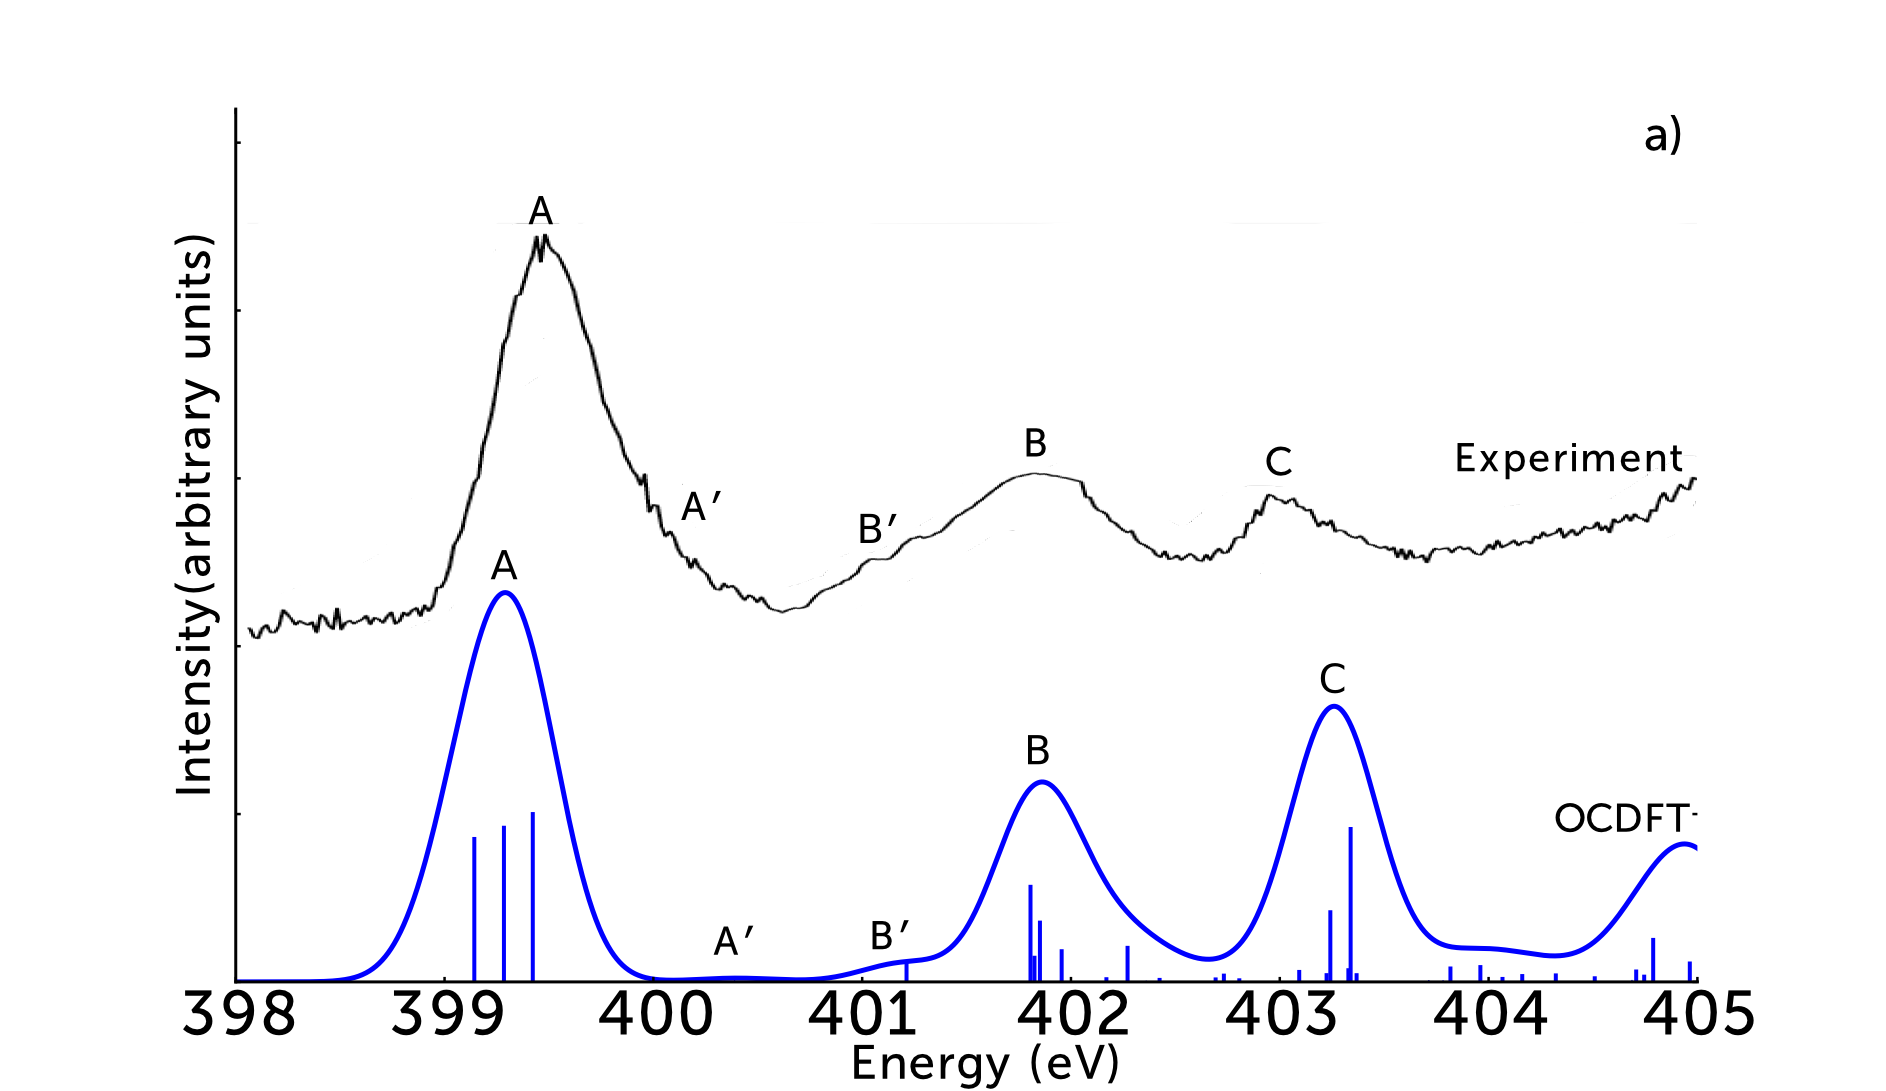
\includegraphics[width=8.8cm]{AdenineNKexperiment.png} \\
%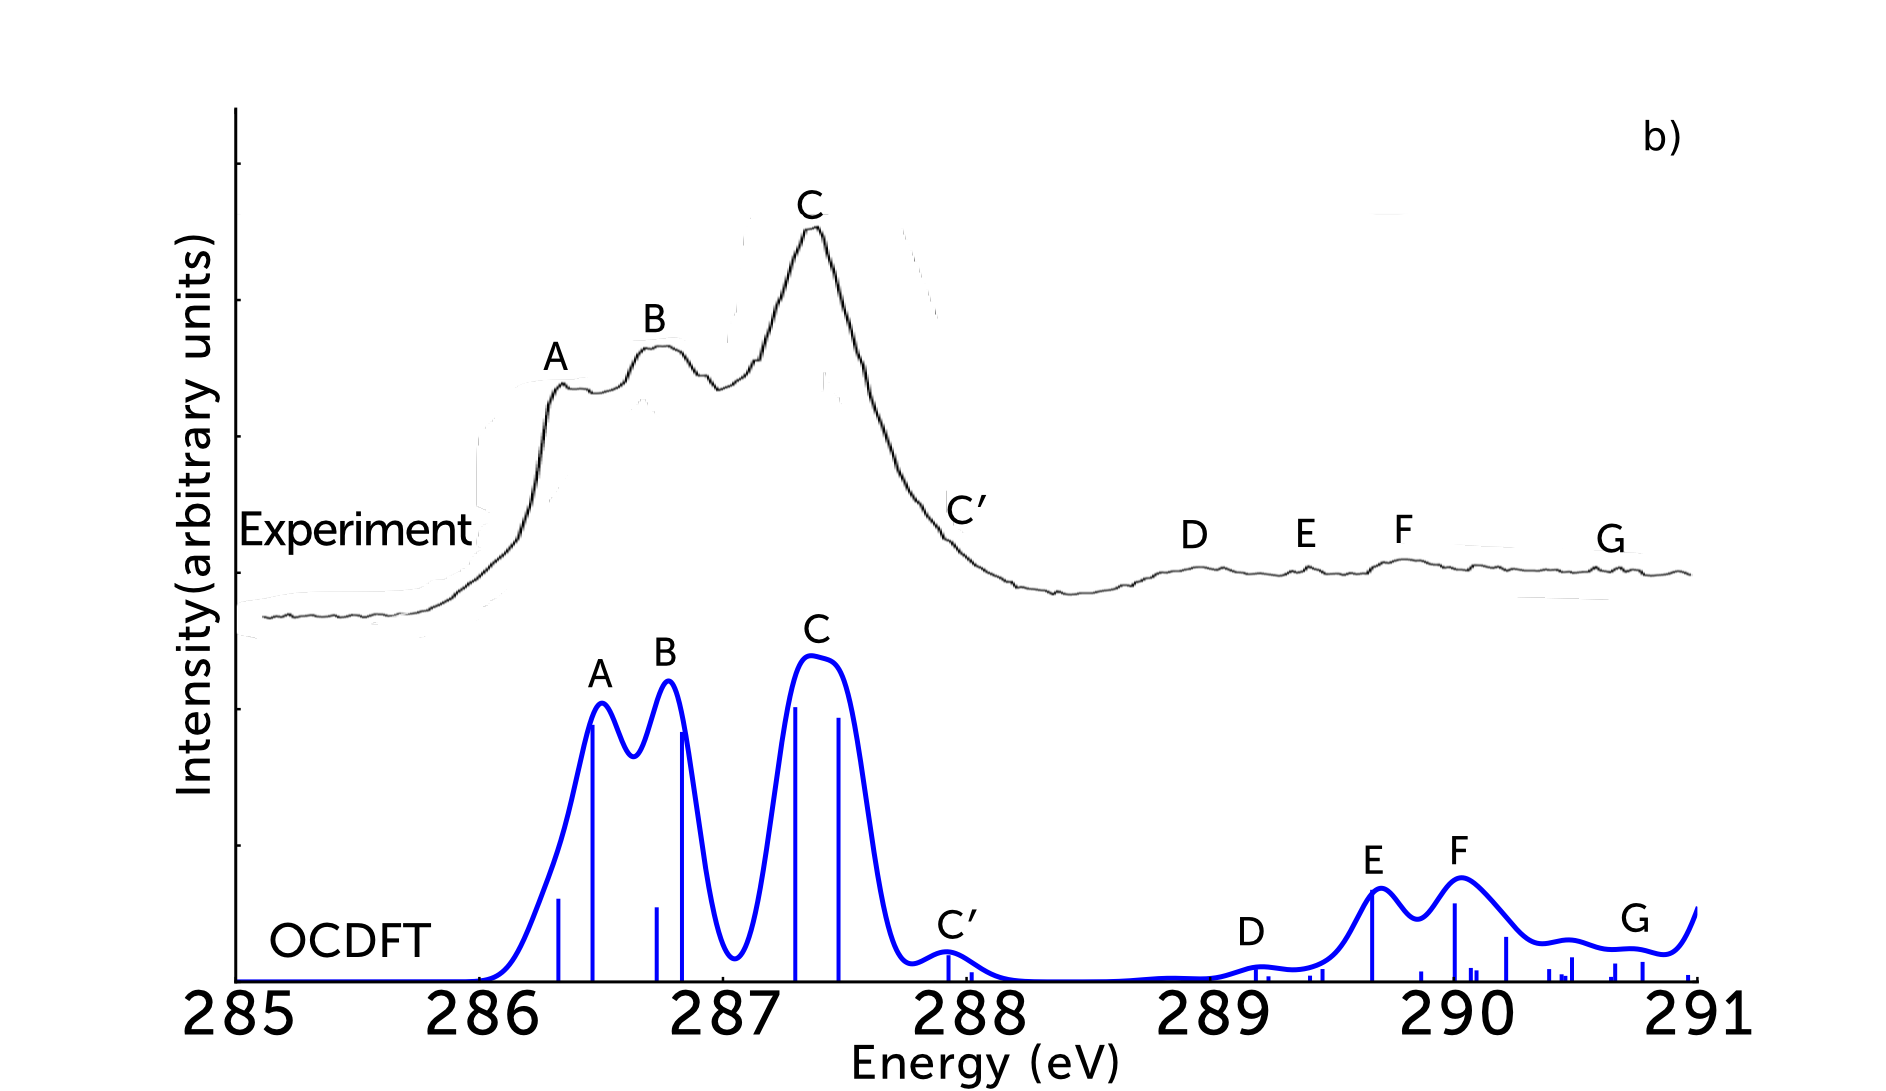
\includegraphics[width=8.8cm]{AdenineCKexperiment.png}
\caption{Core excited states for adenine computed using B3LYP functional and def2-TZVP basis set. Spectra is composed of convoluted Gaussians with a specified Full-Width at Half Maximum (FWHM) of the (a) nitrogen K-edge (FWHM = 0.2 eV) and (b) carbon K-edge (FWHM = 0.2 eV).}
\label{figure:Adenine}
\end{figure} 
\subsubsection{Adenine Nitrogen K-Edge}
   \ Figure \ref{figure:Adenine}a displays the nitrogen k-edge of adenine computed with OCDFT. The most dominant feature of the spectra, Peak A, is experimentally classified at 399.5 eV, our calculations show that this feature is a result of core-valence excitations originating from three of the four nitrogens on the purine ring system (N$_4$, N$_3$, N$_5$). The largest contributor being a transition from N$_5$ $\rightarrow$ $\pi_2^*$ predicted at 399.42, which agrees well with the experimental classification for the peak. An apparent shoulder feature with fairly weak oscillator strength is present in the experimental spectra in the region from 399.8 - 400.4 eV. We represent this feature well, with two weak $\pi^*$ resonances resulting from the two nitrogens on the six-membered ring. A few rising shoulder features are shown in the experimental spectra in the region from 401.0 eV - 401.3 eV, OCDFT predicts a N$_3$ $\rightarrow$ $\pi^*$ transition in this region with a relative oscillator strength of 0.109. Peak B is a mixture of transition to $\pi^*$ orbitals as well as diffuse orbitals. The prominent contributors are $\pi^*$ resonances with the N$_1$ $\rightarrow$ $\pi^*$ being the most intense at 401.81 eV. This is commensurate to the experimental peak assignment at 401.9, the peak height relative to peak A is also in good agreement with experiment. The experimental spectra shows a relatively weak resonance around 403.0 (peak C).  We predict that the dominant contributor to peak C is a transition from N$_2$ $\rightarrow$ D$_6$, the intensity of which, that rivals the strongest transition (f$_{\rm rel}$ = 0.918). This peak intensity is contrary to the experimental spectra which shows peak C  as a superposition of weak transitions. The highest energy transitions are all weak transitions to mostly orbitals of diffuse character. The experimental spectra shows that these transitions get more intense as they appraoch 405.0 eV, which is represented well in our calculations. \\
The experimental carbon k-edge for adenine is dominated by a large single band with three distinct resonances in the low energy regime. \\
 \begin{table}
 \footnotesize
 \centering
     \begin{tabular}{c@{\hskip 0.22in}c@{\hskip 0.22in}c@{\hskip 0.22in}c@{\hskip 0.52in}c@{\hskip 0.22in}c@{\hskip 0.22in}c}
     \hline
     \hline
   \multicolumn{4}{c}{OCDFT} &\multicolumn{2}{c}{Experiment} \\
   \hline
 $\phi_h$ &  $\phi_p$ & $\omega_{fi}$ & f$_{rel}$ & Peak &  $\omega_{fi}$   \\
   \hline
    N$_4$
 &   81.0$\%$ $\pi_1^*$  & 399.14 & 0.851 & \multirow{3}{*}{A} & \multirow{3}{*}{399.5} \\
    N$_3$
 &   63.7$\%$ $\pi_1^*$  & 399.28 & 0.926 \\
    N$_5$
 &   92.6$\%$ $\pi_2^*$  & 399.42 & 1.000 
\vspace{0.05in}\\
    N$_5$
 &   92.4$\%$ $\pi_1^*$  & 399.69 & 0.002 & \multirow{2}{*}{A$^{\prime}$} & \multirow{2}{*}{$\approx$ 400.4}  \\
    N$_4$
 &   98.9$\%$ $\pi_2^*$
 & 400.39 & 0.022 
 \vspace{0.05in}\\
    N$_3$
 &   81.6$\%$ $\pi_2^*$  & 401.21 & 0.109 & B$^{\prime}$ & 401.3 
 \vspace{0.05in}\\
    N$_2$
 &   82.1$\%$ $\pi_1^*$  & 401.43 & 0.364 & \multirow{3}{*}{B} & \multirow{3}{*}{401.9}\\
    N$_1$
 &   69.3$\%$ $\pi_1^*$  & 401.81 & 0.594 \\
    N$_2$
 &   78.4$\%$ $\rm D_3$  & 402.27 & 0.204
 \vspace{0.05in}\\ 
    N$_1$
 &   74.8$\%$ $\pi_2^*$  & 403.08 & 0.122 & \multirow{3}{*}{C} & \multirow{3}{*}{403.0} \\
    N$_1$
 &   87.2$\%$ $\rm D_2$  & 403.25 & 0.418 \\
    N$_2$
 &   57.1$\%$ $\rm D_6$  & 403.34 & 0.918
 \vspace{0.05in}\\
 \hline
 \hline
   \end{tabular}
   \caption{Calculated and experimental adenine nitrogen core excitation energies in eV are shown in the table. All computations are performed using the def2-TZVP basis set and B3LYP functional. The largest contribution to the particle orbital ($\phi_p$) with reference to the ground state valence set is reported along with the hole orbital ($\phi_h$) for each transition. Relative oscillator strengths (f$_{rel}$) are also reported}
 \label{fig: adenine_k_nitrogen}
 \end{table}
\subsubsection{Adenine Carbon K-Edge}
\begin{figure*}[!ht]
\centering
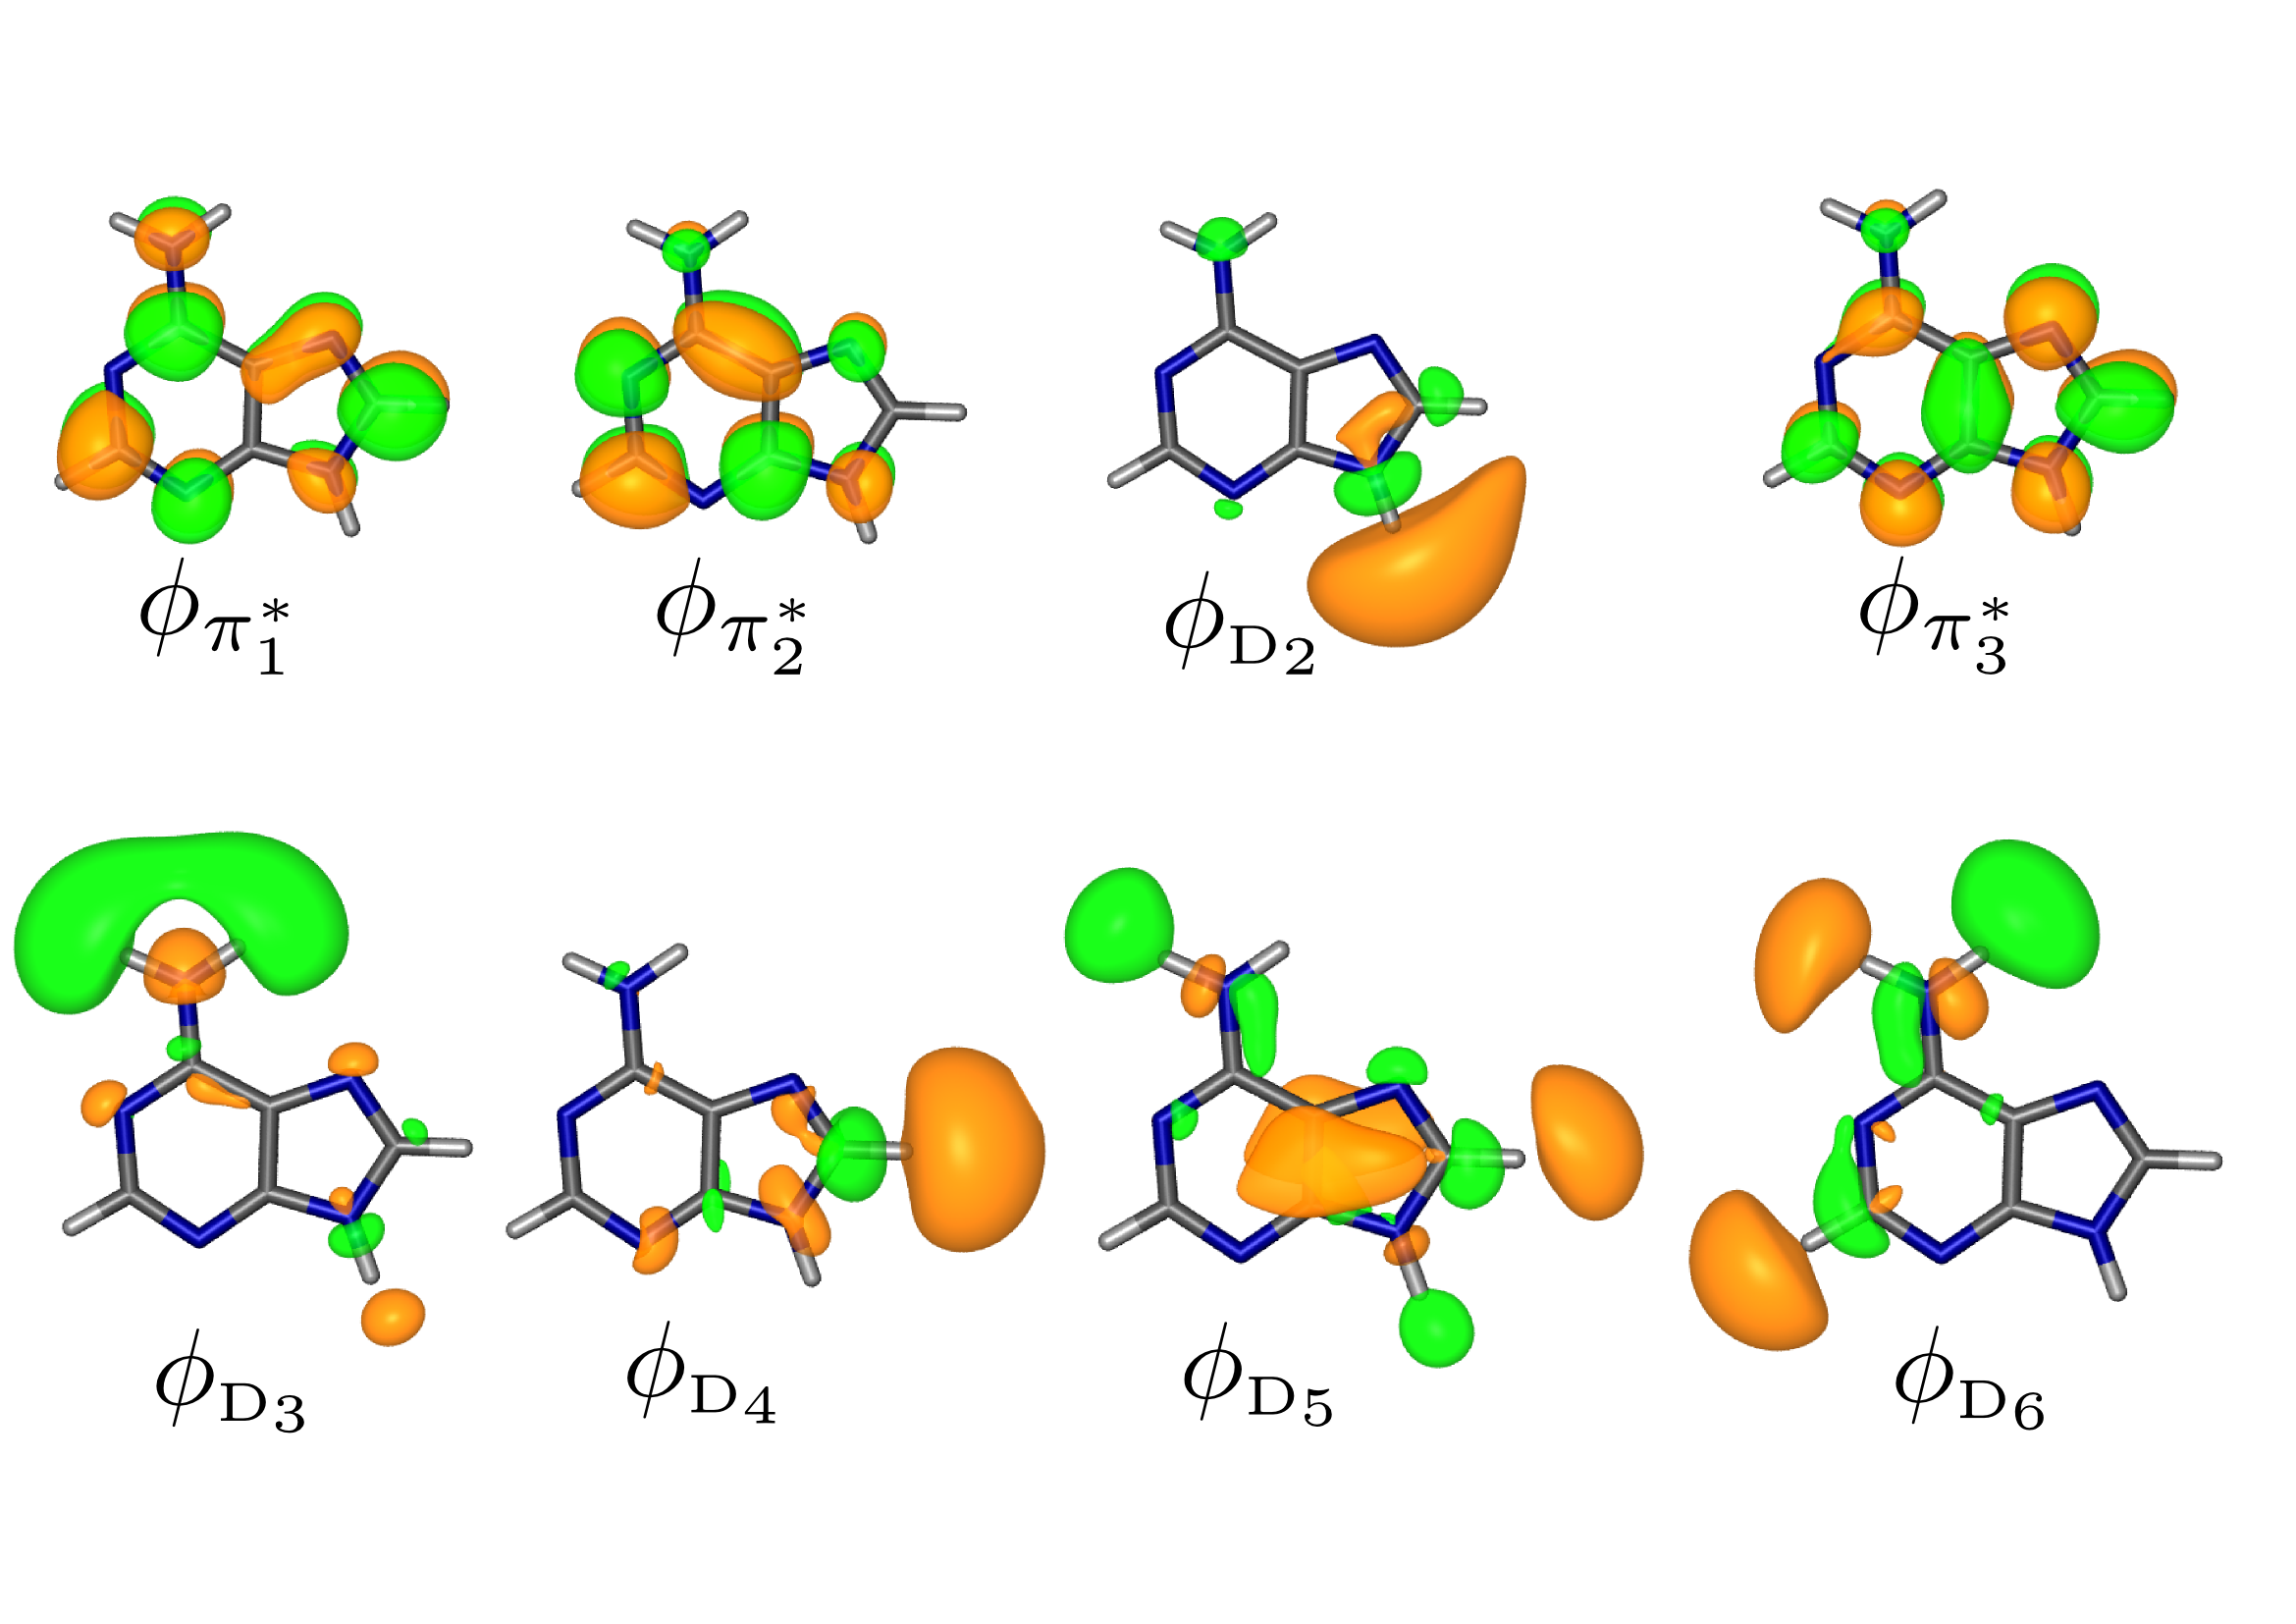
\includegraphics[width=14cm]{AdenineVirtuals.png} \\
\caption{Relevant virtual orbitals for adenine numbered in order based on orbital energy. Orbitals with obvious $\pi^*$ character are labeled as such, while orbitals where electron density is mostly diffused on the outside of the molecule are labeled as $\phi_D$.}
\label{figure:Adenine} 
\end{figure*}
Figure \ref{figure:Adenine}b displays the carbon k-edge of adenine computed with OCDFT in comparison to the experimental results. The theoretical spectra shows peaks A and B, blending together into a single band, the experimental spectra shows these peaks at similar intensities, with peak B being slightly more intense, this is represented well in our calculated spectra. Peak A has a maximum located at 286.4 eV in the experimental spectra, our calculations agree well with this predicting a transition from C$_9$ $\rightarrow$ $\pi_1^*$ at 286.46 eV as the dominant contributor. Similar agreement is seen with peak B located at 286.8 eV, with OCDFT predicting it's dominant contributor to be a transition from C$_7$ $\rightarrow$ $\pi_1^*$.  The OCDFT spectra predicts peak C as the most intense spectral feature, which is consistent with experiment. However, the oscillator strength is inconsistent with experimental peak intensities, according to the experimental results this peak should be roughly 3 times more intense than the adjacent peak B. OCDFT predicts that the C$_6$ $\rightarrow$ $\pi^*_1$ that dominates peak C is only slightly more intense than the dominant contributions to peaks A and B. A very weak shoulder feature is present on the falling edge of peak C, we denote this feature as C$^{\prime}$ and it is represented well by OCDFT. This shoulder results from $\pi^*$ transitions with hole orbitals located on the bridge carbons (C$_8$ and C$_{10}$) and a carbon located on the six-member ring (C$_9$). Peaks D-G were not given experimental peak assignments due to the low intensities of the transitions involved. Peak D is a very weak spectral feature with dominant contributions from excitations to diffuse orbital D$_3$. Peaks E and F are also weak spectral features resulting mostly from transitions to diffuse orbitals. Every transition with energy higher than peak F is extremely weak \\
 \begin{table}
  \footnotesize
 	\centering
     \begin{tabular}{c@{\hskip 0.22in}c@{\hskip 0.22in}c@{\hskip 0.22in}c@{\hskip 0.52in}c@{\hskip 0.22in}c@{\hskip 0.22in}c}
     \hline
     \hline
   \multicolumn{4}{c}{OCDFT} &\multicolumn{2}{c}{Experiment} \\
   \hline
 $\phi_h$ &  $\phi_p$ & $\omega_{fi}$ & f$_{rel}$ & Peak &  $\omega_{fi}$   \\
   \hline
    C$_{10}$
 &   92.6$\%$ $\pi_2^*$  & 286.32 & 0.298 & \multirow{2}{*}{A} & \multirow{2}{*}{286.4}\\
    C$_9$
 &   81.0$\%$ $\pi_1^*$  & 286.46 & 0.936 
 \vspace{0.05in}\\
    C$_{10}$
 &   92.4$\%$ $\pi_1^*$  & 286.71 & 0.260 &  \multirow{2}{*}{B} &  \multirow{2}{*}{286.8} \\
    C$_7$
 &   82.1$\%$ $\pi_1^*$  & 286.86 & 0.893 
 \vspace{0.05in}\\
    C$_6$
 &   69.3$\%$ $\pi_1^*$  & 287.27 & 1.000 &  \multirow{2}{*}{C} &  \multirow{2}{*}{287.4}\\
    C$_8$
 &   63.7$\%$ $\pi_1^*$  & 287.41 & 0.961 
 \vspace{0.05in}\\
    C$_8$
 &   81.6$\%$ $\pi_2^*$  & 287.86 & 0.000 &  \multirow{3}{*}{C$^{\prime}$} &  \multirow{3}{*}{$\approx$ 288.0}\\
    C$_{10}$
 &   34.7$\%$ $\pi_3^*$  & 287.93 & 0.092 \\
    C$_9$
 &   98.9$\%$ $\pi_2^*$
 & 288.02 & 0.026 
 \vspace{0.05in}\\
    C$_6$
 &   74.8$\%$ $\pi_2^*$  & 288.78 & 0.008 & \multirow{3}{*}{D} & \multirow{3}{*}{289.0} \\
    C$_{10}$
 &   36.4$\%$ $\rm D_3$  & 289.16 & 0.038 \\
    C$_8$
 &   66.2$\%$ $\pi_3^*$  & 289.21 & 0.014 
 \vspace{0.05in}\\
    C$_9$
 &   77.4$\%$ $\pi_3^*$  & 289.41 & 0.016 & \multirow{3}{*}{E} \\
    C$_7$
 &   87.1$\%$ $\pi_2^*$  & 289.43 & 0.042 \\
    C$_7$
 &   57.1$\%$ $\rm D_6$  & 289.66 & 0.329 
 \vspace{0.05in}\\ 
    C$_9$
 &   80.2$\%$ $\rm D_2$  & 289.98 & 0.266 & \multirow{5}{*}{F} \\
    C$_8$
 &   90.2$\%$ $\rm D_2$  & 290.06 & 0.044 \\
    C$_9$
 &   83.4$\%$ $\rm D_3$  & 290.14 & 0.166
 \vspace{0.05in}\\
    C$_7$
 &   94.8$\%$ $\pi_3^*$  & 290.36 & 0.086  & \multirow{3}{*}{G} \\
    C$_6$
 &   77.2$\%$ $\pi_3^*$  & 290.66 & 0.060 \\
    C$_7$
 &   56.6$\%$ $\rm D_2$  & 290.77 & 0.064 \\
 \hline
 \hline
   \end{tabular}
      \caption{Calculated and experimental adenine carbon core excitation energies in eV are shown in the table. All computations are performed using the def2-TZVP basis set and B3LYP functional. The largest contribution to the particle orbital ($\phi_p$) with reference to the ground state valence set is reported along with the hole orbital ($\phi_h$) for each transition. Relative oscillator strengths (f$_{rel}$) are also reported}
   \label{table: adenine_k_carbon}
   \end{table}
\subsubsection{Comparison With ADC(2) Calculations} \
Previous theoretical studies performed using ADC(2) provide a good basis of comparison for the performance of the OCDFT spectra. Three key differences in the spectra are noted here. 
The shoulder feature B$^{\prime}$ in the thymine oxygen K-Edge shown in Fig. \ref{figure:Thymine} is completely absent from the ADC(2) spectra[CITE]. However, a more recent study by Wenzel, Wormit, and Dreuw [CITE] uses a core-valence separation (CVS) approximation to the ADC(2) working equations [CVS-ADC(2)] and predicts three excitations in this shoulder region B$^{\prime}$, all with f$_{abs}$ $<$ 0.001. These weaker oscillator strengths predicted by CVS-ADC(2) are more consistent with the experimental peak profile. \\ 
The overall shape of the OCDFT thymine K-Edge is more consistent with the experimental excitation manifold than the ADC(2) spectra. The two peaks A and B in Fig. \ref{figure:Thymine}b have clear, distinct maxima which are produced well quantitatively with ADC(2) (after applying a uniform shift of -2.59 eV to the spectra), strong $\pi^*$ resonances are reported near both experimental peak maxima. However, the contour of the peak is inconsistent with the experimental manifold. The ADC(2) spectra blends into one large spectral band over the interval from 401.0 eV to 404.5 eV encompassing very closely spaced transitions, all with relatively high oscillator strengths. The extremely tight spacings and high intensities of these transitions seem to be present even in the updated CVS-ADC(2) results. The OCDFT spectra doest not suffer from this single band issue, as the $\pi^*$ resonances in peak A are well separated from the strong 3s Rydberg transitions in peak B by more than 1.0 eV. The agreement of these results with experiment, suggest that this picture of well-separated $\pi^*$ and Rydberg resonances is more congruous with reality. However, a more detailed study into the nitrogen core excitation manifold of thymine would be required prove this to be true, and is outside of the scope of this current study. \\
ADC(2) was unable to fully resolve peaks B$^{\prime}$, B, and C in the adenine nitrogen edge shown in Fig. \ref{figure:Adenine}a. The OCDFT spectra represents these peaks well, as separated spectral features, in compliance with the experimental structure. While ADC(2) reports a spectra where these three features merge into a single band structure. 
\begin{comment}
  \begin{figure}[ht!]
  \centering
  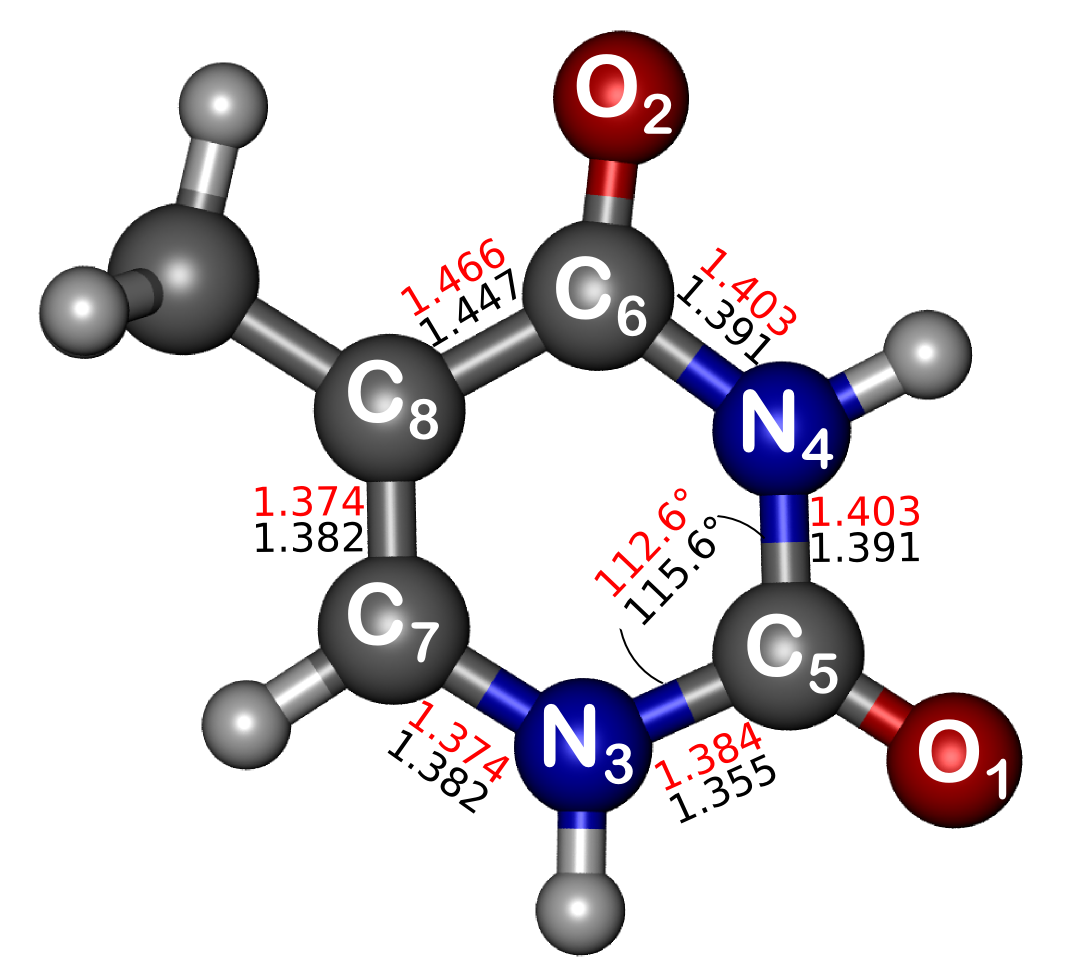
\includegraphics[scale=0.50]{g130.png}
  \caption{Optimized geometry and numbering scheme for thymine. Atoms are numbered based on the Khon--Sham orbital energy of their respective 1s orbitals starting with the minimum energy core (O$_1$). The top number (in red) is the calculated bond length ($\AA$)/angle (degrees) computed at the B3LYP level of theory, while the bottom number (in black) shows values from the experimental crystal structure.[CITE]}
  \end{figure}
\end{comment}
    \begin{comment}
The position of spectral features computed with OCDFT are in excellent agreement with experiment. At this time the limitations of the MCHP algorithm make it possible to only compute the valence states of a molecules like thymine and adenine with little to no symmetry. With the smaller, symetrical molecules in our test set, it was possible to exploit symmetry in order to obtain the Rydberg states, but that isn't possible with nonsymmetrical molecules. However, since most K-edge spectra have strong features arising from excitations to valence antibonding orbitals[CITE], it is still possible to evaluate the accuracy of OCDFT in simulating spectral features. Theoretical line intensities were approximated using the oscillator stengths computed in OCDFT. The excited state orbitals shown in Figure \ref{figure:MOs} are the two unique molecular orbitals from thymine. The most likely excited state orbital chosen by the MCHP algorithm depends on the spatial orientation of the core orbital. Almost all core orbitals are excited to $\pi_1^*$ while the 1s orbitals from O$_1$ and C$_5$ are excited to $\pi_2^*$ using this procedure. Due to the projective nature of the algorithm, it is not possible to obtain the other valence states, Rydberg states, or mixed valence/Rydberg states without exploiting symmetry, which is not helpful for a molecule like Thymine. Thus at this time it is only possible to obtain the excitations from the respective 1s orbital and its closest valence orbital. 
\end{comment}
   \begin{comment}
\noindent The computed oxygen K-edge shown in Figure \ref{figure:Thymine}a is in good agreement with the experimental peaks. The two most dominant features of this spectra are excitations from the respective O 1s orbitals, to $\pi^*$ particle orbitals. The MCHP algorithm is able to reproduce these features well. The energy region above 534 eV is dominated by Rydberg transitions and mixed valence/Rydberg states and therefore is outside the scope of the current study. The most prominent feature of the experimental N K-edge shown in Figure \ref{figure:Thymine}b is the large peak near 403 eVs. This peak is a mix of valence and Rydberg excitations from the N$_3$ 1s and N$_4$ 1s orbitals, however because of the projective nature of the algorithm we are unable to calculate these states at this time. Peak C at 401.6 eVs is in excellent agreement with the experimental peak maximum around 401.7 eVs. The N 1s excitation manifold is complex, the experimental spectra is cluttered with multiple transitions within a small region. This makes it difficult to clarify exactly which experimental peak that D corresponds to, but we can compare our value to the same transition calculated using ADC(2) (See table in Figure \ref{figure:MOs} for details). Figure \ref{figure:Thymine}c shows that the computed C K-edge is in excellent agreement with experimental spectra. All of the prominent features of this spectra are excitations from C 1s orbitals to the $\pi^*$ particle orbitals. The computed line intensities are very similar to the experimental spectra giving us great confidence in the ability of OCDFT to compute the oscillator strengths of core-valence excited states.
Figure \ref{figure:Adenine} displays the nitrogen and carbon K-edges of adenine computed with OCDFT. Peak A, the most prominent feature of the spectra, contains contributions from three of the nitrogen atoms located on the ring system. Since peak A is composed entirely of valence excitations from unique 1s core orbitals, this is the best glimpse at the accuracy of OCDFT when it is able to calculate all peak contributions. The peak of the Gaussian formed by all contributions to the peak is centered around 399.3 eV, very close to the experimental peak centered at 399.5 eV. The relative line intensity, when compared to peaks B and C, is almost identical to the relative intensity seen in the experimental spectra. Peak B is largely a shoulder feature of peak C, and this relationship is captured perfectly in our theoretical spectra. The experimental peak at 403 eV is composed of Rydberg excitations from N$_3$ and N$_4$, outside the scope of the MCHP algorithm. The carbon K-edge is also in good agreement, once again we see a spectra whose main features can be captured without considering the Rydberg states. The three main peaks between 286 eV and 288 eV are well represented by OCDFT. The line intensity of peak F is replicated well, although the intensities of peaks D and E differ slightly from experiment. \\
\end{comment}
\section{Conclusions}
Orthogonality constrained density functional theory represents a new frontier in simulating excited states using density functional methods. Many of the efforts in this field have centered around developing new functionals in order to compensate for the shortcomings of the standard GGA functionals by varying the amount of hartree-fock exchange and other semi-empirical parameters. Previous studies done using time dependent density functional methods have all concluded that the 20-25\% hartree-fock exchange present in many standard hybrid functionals is not sufficient enough to describe core-excited states using TDDFT. However, here we show that standard functionals perform well with OCDFT at computing core-excited states due to the local nature of the integrals present in the excitation energy expression that allow for a better description of core-valence excitations. We have proven this by benchmarking OCDFT over a range of first and second row core excitations using conventional pure and hybrid functionals. OCDFT showed no significant dependence on the amount of HF exchange, producing similar results across different functionals with varying fractions of HF exchange. OCDFT also performed well across both the first and second row of the periodic table, only losing approximately 1.0 eV of accuracy when moving to the second row of the periodic table. Also outperforming TDDFT by ~11.1 eV when calculating first row core excitations, and by ~30.0 eV when calculating second row core excitations. We also calculate the NEXAS spectra of thymine and adenine to show that OCDFT produces an accurate spectra without the aid of a corrective energy shift. Calculated oscillator strengths are in excellent agreement with the experimental peak intensities, confirming that OCDFT is effective at calculating transition dipole moments. Our calculations show distinct $\pi^*$ transitions in the lower energy regime and significant mixing between the $\pi^*$ and diffuse orbitals in the higher energy regime of the spectra, which agrees well with previous NEXAS studies of these molecules.
\section{Supplementary}
   \begin{table}
 \centering
     \begin{tabular}{c@{\hskip 0.22in}c@{\hskip 0.22in}c@{\hskip 0.22in}c@{\hskip 0.52in}c@{\hskip 0.22in}c@{\hskip 0.22in}c}
     \hline
     \hline
   \multicolumn{4}{c}{OCDFT} &\multicolumn{2}{c}{Experiment} \\
   \hline
 $\phi_h$ &  $\phi_p$ & $\omega_{fi}$ & f$_{rel}$ & Peak &  $\omega_{fi}$   \\
   \hline
    O$_2$
 &   81.8$\%$ $\pi_1^*$  & 531.05 & 1.000 & A  & 531.4
 \vspace{0.1in}\\
    O$_1$
 &   64.0$\%$ $\pi_2^*$  & 532.08 & 0.968 & B & 532.3
 \vspace{0.1in}\\
    O$_1$
 &   71.2$\%$ $\pi_1^*$  & 533.38 & 0.146 & \multirow{2}{*}{B$^{\prime}$} & \multirow{2}{*}{$\approx$ 533.8}  \\
    O$_2$
 &   78.3$\%$ $\pi_2^*$  & 533.75 & 0.162 
 \vspace{0.1in}\\
    O$_1$
 &   77.0$\%$ $\rm D_1$  & 534.74 & 0.008  & \multirow{9}{*}{C} & \multirow{9}{*}{535.7} \\
    O$_2$
 &   65.9$\%$ $\rm D_1$  & 534.85 & 0.042 \\
    O$_2$
 &   44.1$\%$ $\rm D_3$  & 535.28 & 0.020 \\
    O$_1$
 &   69.5$\%$ $\rm D_3$  & 535.46 & 0.098 \\
    O$_2$
 &   60.8$\%$ $\rm D_2$  & 535.53 & 0.085 \\
    O$_1$
 &   76.0$\%$ $\pi_3^*$  & 536.12 & 0.222 \\
    O$_2$
 &   69.0$\%$ $\pi_3^*$  & 536.24 & 0.104 \\
    O$_2$
 &   86.3$\%$ $\rm D_4$  & 536.34 & 0.052 \\
    O$_1$
 &   76.3$\%$ $\rm D_2$  & 536.60 & 0.039 
 \vspace{0.1in}\\
    O$_2$
 &   44.4$\%$ $\rm D_6$  & 537.02 & 0.024 & \multirow{6}{*}{D} & \multirow{6}{*}{537.1} \\
    O$_1$
 &   83.5$\%$ $\rm D_4$  & 537.10 & 0.047 \\
    O$_2$
 &   63.7$\%$ $\rm D_5$  & 537.21 & 0.021 \\
    O$_1$
 &   35.6$\%$ 42-A  & 537.45 & 0.054 \\
    O$_2$
 &   44.0$\%$ 42-A  & 537.67 & 0.073 \\
    O$_1$
 &   43.6$\%$ $\rm D_5$  & 537.72 & 0.036 
 \vspace{0.1in}\\
    O$_1$
 &   70.7$\%$ $\rm D_6$  & 538.49 & 0.058 \\
   \end{tabular}
         \caption{Calculated and experimental thymine oxygen core excitation energies in eV are shown in the table. All computations are performed using the def2-TZVP basis set and B3LYP functional. The largest contribution to the particle orbital ($\phi_p$) with reference to the ground state valence set is reported along with the hole orbital ($\phi_h$) for each transition. Relative oscillator strengths (f$_{rel}$) are also reported}
   \label{table: thymine_k_oxygen}
   \end{table}
        \begin{table}
 \centering
     \begin{tabular}{c@{\hskip 0.22in}c@{\hskip 0.22in}c@{\hskip 0.22in}c@{\hskip 0.52in}c@{\hskip 0.22in}c@{\hskip 0.22in}c}
     \hline
     \hline
   \multicolumn{4}{c}{OCDFT} &\multicolumn{2}{c}{Experiment} \\
   \hline
 $\phi_h$ &  $\phi_p$ & $\omega_{fi}$ & f$_{rel}$ & Peak &  $\omega_{fi}$   \\
   \hline
    N$_4$
 &   81.8$\%$ $\pi_1^*$  & 401.18 & 1.000 & \multirow{2}{*}{A} & \multirow{2}{*}{401.7} \\
    N$_3$
 &   64.0$\%$ $\pi_2^*$  & 401.76 & 0.805 
 \vspace{0.1in}\\
    N$_4$
 &   78.3$\%$ $\pi_2^*$  & 402.50 & 0.087 & \multirow{3}{*}{B} & \multirow{3}{*}{402.7}\\
    N$_3$
 &   77.0$\%$ $\rm D_1$  & 403.09 & 0.863 \\
    N$_4$
 &   65.9$\%$ $\rm D_1$  & 403.33 & 0.765 
 \vspace{0.1in}\\
    N$_4$
 &   44.1$\%$ $\rm D_3$  & 404.17 & 0.912 & C & 404.1 
 \vspace{0.1in}\\
    N$_4$
 &   60.8$\%$ $\rm D_2$  & 404.94 & 0.144 & \multirow{7}{*}{D} & \multirow{6}{*}{405.5}\\
    N$_3$
 &   69.5$\%$ $\rm D_3$  & 405.09 & 0.374 \\
    N$_4$
 &   86.3$\%$ $\rm D_4$  & 405.31 & 0.864 \\
    N$_3$
 &   76.0$\%$ $\pi_3^*$  & 405.41 & 0.333 \\
    N$_4$
 &   69.0$\%$ $\pi_3^*$  & 405.62 & 0.183 \\
    N$_3$
 &   71.2$\%$ $\pi_1^*$  & 405.67 & 0.490 \\
    N$_3$
 &   76.3$\%$ $\rm D_2$  & 405.76 & 0.177 \\
 \end{tabular}
  \caption{Calculated and experimental thymine nitrogen core excitation energies in eV are shown in the table. All computations are performed using the def2-TZVP basis set and B3LYP functional. The largest contribution to the particle orbital ($\phi_p$) with reference to the ground state valence set is reported along with the hole orbital ($\phi_h$) for each transition. Relative oscillator strengths (f$_{rel}$) are also reported}
   \label{table: thymine_k_nitrogen}
 \end{table}
      \begin{table}
 \centering
     \begin{tabular}{c@{\hskip 0.22in}c@{\hskip 0.22in}c@{\hskip 0.22in}c@{\hskip 0.52in}c@{\hskip 0.22in}c@{\hskip 0.22in}c}
     \hline
     \hline
   \multicolumn{4}{c}{OCDFT} &\multicolumn{2}{c}{Experiment} \\
   \hline
 $\phi_h$ &  $\phi_p$ & $\omega_{fi}$ & f$_{rel}$ & Peak &  $\omega_{fi}$   \\
   \hline
    C$_8$
 &   92.1$\%$ $\pi_1^*$  & 284.90 & 0.372 & A & 284.9  
 \vspace{0.1in} \\
    C$_7$
 &   95.9$\%$ $\pi_1^*$  & 285.98 & 0.698 & B & 285.9
 \vspace{0.1in} \\
    C$_9$
 &   75.4$\%$ $\pi_2^*$  & 286.56 & 0.036 & \multirow{5}{*}{C} & \multirow{5}{*}{287.8} \\
    C$_8$
 &   97.6$\%$ $\pi_2^*$  & 287.33 & 0.171 \\
    C$_6$
 &   81.8$\%$ $\pi_1^*$  & 287.68 & 0.792 \\
    C$_9$
 &   89.9$\%$ $\pi_1^*$  & 287.92 & 0.117 \\
    C$_8$
 &   48.1$\%$ $\rm D_3$  & 288.19 & 0.006 
 \vspace{0.1in} \\
    C$_9$
 &   87.7$\%$ $\rm D_1$  & 288.46 & 0.229 & \multirow{9}{*}{D} & \multirow{9}{*}{289.4} \\
    C$_8$
 &   53.9$\%$ $\rm D_1$  & 288.94 & 0.037 \\
    C$_9$
 &   85.1$\%$ $\rm D_3$  & 289.01 & 0.158 \\
    C$_7$
 &   94.2$\%$ $\pi_2^*$  & 289.06 & 0.289 \\
    C$_5$
 &   64.0$\%$ $\pi_2^*$  & 289.14 & 1.000 \\
    C$_8$
 &   32.5$\%$ $\rm D_3$  & 289.17 & 0.017 \\
    C$_7$
 &   90.3$\%$ $\rm D_1$  & 289.22 & 0.001 \\
    C$_9$
 &   63.1$\%$ $\pi_3^*$  & 289.26 & 0.333 \\
    C$_9$
 &   49.5$\%$ $\rm D_2$  & 289.31 & 0.375 
 \vspace{0.1in}\\
    C$_8$
 &   67.1$\%$ $\rm D_2$  & 289.67 & 0.082 \\
    C$_8$
 &   77.0$\%$ $\rm D_4$  & 289.68 & 0.105 \\
    C$_6$
 &   78.3$\%$ $\pi_2^*$  & 289.94 & 0.135 
 \vspace{0.1in}\\
    C$_9$
 &   75.4$\%$ $\rm D_4$  & 290.14 & 0.023 & \multirow{6}{*}{E} &  \multirow{6}{*}{290.7} \\
    C$_8$
 &   33.3$\%$ $\rm D_5$  & 290.31 & 0.119 \\
    C$_5$
 &   71.2$\%$ $\pi_1^*$  & 290.33 & 0.029 \\
    C$_9$
 &   30.5$\%$ $\rm D_5$  & 290.43 & 0.047 \\
    C$_7$
 &   71.6$\%$ $\rm D_3$  & 290.44 & 0.050 \\
    C$_7$
 &   41.5$\%$ $\rm D_2$  & 290.54 & 0.041 
 \vspace{0.1in}\\
    C$_8$
 &   38.1$\%$ $\rm D_6$  & 290.80 & 0.093 \\
    C$_9$
 &   24.4$\%$ $\rm D_6$  & 291.12 & 0.076 \\
    C$_8$
 &   61.2$\%$ 42-A  & 291.13 & 0.024 \\
    C$_7$
 &   45.5$\%$ $\pi_3^*$  & 291.42 & 0.018 \\
    C$_7$
 &   83.1$\%$ $\rm D_4$  & 291.44 & 0.001 \\
    C$_9$
 &   24.8$\%$ $\rm D_5$  & 291.45 & 0.289 \\
    C$_6$
 &   65.9$\%$ $\rm D_1$  & 291.59 & 0.036 \\
    C$_7$
 &   44.3$\%$ $\rm D_5$  & 291.83 & 0.055 \\
 \end{tabular}
   \caption{Calculated and experimental thymine carbon core excitation energies in eV are shown in the table. All computations are performed using the def2-TZVP basis set and B3LYP functional. The largest contribution to the particle orbital ($\phi_p$) with reference to the ground state valence set is reported along with the hole orbital ($\phi_h$) for each transition. Relative oscillator strengths (f$_{rel}$) are also reported}
   \label{table: thymine_k_carbon}
 \end{table}
  \begin{table}
 \centering
     \begin{tabular}{c@{\hskip 0.22in}c@{\hskip 0.22in}c@{\hskip 0.22in}c@{\hskip 0.52in}c@{\hskip 0.22in}c@{\hskip 0.22in}c}
     \hline
     \hline
   \multicolumn{4}{c}{OCDFT} &\multicolumn{2}{c}{Experiment} \\
   \hline
 $\phi_h$ &  $\phi_p$ & $\omega_{fi}$ & f$_{rel}$ & Peak &  $\omega_{fi}$   \\
   \hline
    N$_4$
 &   81.0$\%$ $\pi_1^*$  & 399.14 & 0.851 & \multirow{3}{*}{A} & \multirow{3}{*}{399.5} \\
    N$_3$
 &   63.7$\%$ $\pi_1^*$  & 399.28 & 0.926 \\
    N$_5$
 &   92.6$\%$ $\pi_2^*$  & 399.42 & 1.000 
\vspace{0.1in}\\
    N$_5$
 &   92.4$\%$ $\pi_1^*$  & 399.69 & 0.002 & \multirow{2}{*}{A$^{\prime}$} & \multirow{2}{*}{$\approx$ 400.4}  \\
    N$_4$
 &   98.9$\%$ $\pi_2^*$
 & 400.39 & 0.022 
 \vspace{0.1in}\\
    N$_3$
 &   81.6$\%$ $\pi_2^*$  & 401.21 & 0.109 & B$^{\prime}$ & 401.3 
 \vspace{0.1in}\\
    N$_2$
 &   82.1$\%$ $\pi_1^*$  & 401.43 & 0.364 & \multirow{9}{*}{B} & \multirow{9}{*}{401.9}\\
    N$_3$
 &   66.2$\%$ $\pi_3^*$  & 401.79 & 0.145 \\
    N$_1$
 &   69.3$\%$ $\pi_1^*$  & 401.81 & 0.594 \\
    N$_4$
 &   77.4$\%$ $\pi_3^*$  & 401.95 & 0.184 \\
    N$_5$
 &   56.7$\%$ $\pi_3^*$  & 402.10 & 0.017 \\
    N$_5$
 &   34.7$\%$ $\pi_3^*$  & 402.15 & 0.013 \\
    N$_2$
 &   78.4$\%$ $\rm D_3$  & 402.27 & 0.204 \\
    N$_4$
 &   80.2$\%$ $\rm D_2$  & 402.36 & 0.003 \\
    N$_3$
 &   90.2$\%$ $\rm D_2$  & 402.42 & 0.012 
 \vspace{0.1in}\\
    N$_4$
 &   83.4$\%$ $\rm D_3$  & 402.73 & 0.038 & \multirow{10}{*}{C} & \multirow{10}{*}{403.0}\\
    N$_3$
 &   69.0$\%$ $\rm D_3$  & 402.80 & 0.008 \\
    N$_5$
 &   36.4$\%$ $\rm D_3$  & 402.80 & 0.049 \\
    N$_1$
 &   74.8$\%$ $\pi_2^*$  & 403.08 & 0.122 \\
    N$_5$
 &   39.1$\%$ $\rm D_5$  & 403.18 & 0.030 \\
    N$_4$
 &   48.5$\%$ $\rm D_4$  & 403.22 & 0.033 \\
    N$_1$
 &   87.2$\%$ $\rm D_2$  & 403.25 & 0.418 \\
    N$_3$
 &   80.4$\%$ $\rm D_4$  & 403.32 & 0.074 \\
    N$_2$
 &   57.1$\%$ $\rm D_6$  & 403.34 & 0.918 \\
    N$_5$
 &   91.1$\%$ $\rm D_6$  & 403.38 & 0.052 
 \vspace{0.1in}\\
    N$_4$
 &   61.7$\%$ $\rm D_6$  & 403.67 & 0.007 \\
    N$_3$
 &   77.6$\%$ $\rm D_5$  & 403.72 & 0.007 \\
    N$_5$
 &   61.6$\%$ 43-A  & 403.79 & 0.073 \\
    N$_1$
 &   77.2$\%$ $\pi_3^*$  & 403.97 & 0.083 \\
    N$_4$
 &   37.1$\%$ 43-A  & 404.07 & 0.040 \\
    N$_5$
 &   36.3$\%$ $\rm D_4$  & 404.20 & 0.008 \\
    N$_4$
 &   39.8$\%$ 43-A  & 404.24 & 0.022 \\
    N$_2$
 &   94.8$\%$ $\pi_3^*$  & 404.33 & 0.038 \\
    N$_3$
 &   42.3$\%$ 44-A  & 404.44 & 0.023 \\
    N$_2$
 &   87.1$\%$ $\pi_2^*$  & 404.55 & 0.011 \\
    N$_3$
 &   59.8$\%$ $\rm D_6$  & 404.71 & 0.059 \\
    N$_5$
 &   29.0$\%$ $\rm D_5$  & 404.73 & 0.031 \\
    N$_4$
 &   91.9$\%$ 46-A  & 404.79 & 0.253 \\
    N$_2$
 &   56.6$\%$ $\rm D_2$  & 404.97 & 0.115 \\
 \hline
 \hline
   \end{tabular}
   \caption{Calculated and experimental adenine nitrogen core excitation energies in eV are shown in the table. All computations are performed using the def2-TZVP basis set and B3LYP functional. The largest contribution to the particle orbital ($\phi_p$) with reference to the ground state valence set is reported along with the hole orbital ($\phi_h$) for each transition. Relative oscillator strengths (f$_{rel}$) are also reported}
 \label{fig: adenine_k_nitrogen}
 \end{table}
  \begin{table}
 	\centering
     \begin{tabular}{c@{\hskip 0.22in}c@{\hskip 0.22in}c@{\hskip 0.22in}c@{\hskip 0.52in}c@{\hskip 0.22in}c@{\hskip 0.22in}c}
     \hline
     \hline
   \multicolumn{4}{c}{OCDFT} &\multicolumn{2}{c}{Experiment} \\
   \hline
 $\phi_h$ &  $\phi_p$ & $\omega_{fi}$ & f$_{rel}$ & Peak &  $\omega_{fi}$   \\
   \hline
    C$_{10}$
 &   92.6$\%$ $\pi_2^*$  & 286.32 & 0.298 & \multirow{2}{*}{A} & \multirow{2}{*}{286.4}\\
    C$_9$
 &   81.0$\%$ $\pi_1^*$  & 286.46 & 0.936 
 \vspace{0.1in}\\
    C$_{10}$
 &   92.4$\%$ $\pi_1^*$  & 286.71 & 0.260 &  \multirow{2}{*}{B} &  \multirow{2}{*}{286.8} \\
    C$_7$
 &   82.1$\%$ $\pi_1^*$  & 286.86 & 0.893 
 \vspace{0.1in}\\
    C$_6$
 &   69.3$\%$ $\pi_1^*$  & 287.27 & 1.000 &  \multirow{2}{*}{C} &  \multirow{2}{*}{287.4}\\
    C$_8$
 &   63.7$\%$ $\pi_1^*$  & 287.41 & 0.961 
 \vspace{0.1in}\\
    C$_8$
 &   81.6$\%$ $\pi_2^*$  & 287.86 & 0.000 &  \multirow{3}{*}{C$^{\prime}$} &  \multirow{3}{*}{$\approx$ 288.0}\\
    C$_{10}$
 &   34.7$\%$ $\pi_3^*$  & 287.93 & 0.092 \\
    C$_9$
 &   98.9$\%$ $\pi_2^*$
 & 288.02 & 0.026 
 \vspace{0.1in}\\
    C$_6$
 &   74.8$\%$ $\pi_2^*$  & 288.78 & 0.008 & \multirow{5}{*}{D} & \multirow{5}{*}{289.0} \\
    C$_{10}$
 &   56.7$\%$ $\pi_3^*$  & 288.89 & 0.006 \\
    C$_7$
 &   78.4$\%$ $\rm D_3$  & 288.91 & 0.001 \\
    C$_{10}$
 &   36.4$\%$ $\rm D_3$  & 289.16 & 0.038 \\
    C$_8$
 &   66.2$\%$ $\pi_3^*$  & 289.21 & 0.014 
 \vspace{0.1in}\\
    C$_9$
 &   77.4$\%$ $\pi_3^*$  & 289.41 & 0.016 & \multirow{3}{*}{E} \\
    C$_7$
 &   87.1$\%$ $\pi_2^*$  & 289.43 & 0.042 \\
    C$_7$
 &   57.1$\%$ $\rm D_6$  & 289.66 & 0.329 
 \vspace{0.1in}\\
    C$_{10}$
 &   39.1$\%$ $\rm D_5$  & 289.82 & 0.029 & \multirow{5}{*}{F} \\
    C$_9$
 &   80.2$\%$ $\rm D_2$  & 289.98 & 0.266 \\
    C$_8$
 &   90.2$\%$ $\rm D_2$  & 290.06 & 0.044 \\
    C$_9$
 &   83.4$\%$ $\rm D_3$  & 290.14 & 0.166 \\
    C$_6$
 &   87.2$\%$ $\rm D_2$  & 290.15 & 0.035 
 \vspace{0.1in}\\
    C$_7$
 &   94.8$\%$ $\pi_3^*$  & 290.36 & 0.086  & \multirow{8}{*}{G} \\
    C$_{10}$
 &   91.1$\%$ $\rm D_6$  & 290.37 & 0.020 \\
    C$_{10}$
 &   61.6$\%$ 43 - A  & 290.42 & 0.031 \\
    C$_9$
 &   48.5$\%$ $\rm D_4$  & 290.45 & 0.014 \\
    C$_8$
 &   69.0$\%$ $\rm D_3$  & 290.61 & 0.010 \\
    C$_6$
 &   77.2$\%$ $\pi_3^*$  & 290.66 & 0.060 \\
    C$_7$
 &   56.6$\%$ $\rm D_2$  & 290.77 & 0.064 \\
    C$_9$
 &   61.7$\%$ $\rm D_6$  & 290.94 & 0.018 \\
 \hline
 \hline
   \end{tabular}
      \caption{Calculated and experimental adenine carbon core excitation energies in eV are shown in the table. All computations are performed using the def2-TZVP basis set and B3LYP functional. The largest contribution to the particle orbital ($\phi_p$) with reference to the ground state valence set is reported along with the hole orbital ($\phi_h$) for each transition. Relative oscillator strengths (f$_{rel}$) are also reported}
   \label{table: adenine_k_carbon}
   \end{table}
\footnotesize{
\bibliography{OCDFT.bib} %your .bib file
\bibliographystyle{rsc} %the RSC's .bst file
}

\end{document}
